% Format teze zasnovan je na paketu memoir
% http://tug.ctan.org/macros/latex/contrib/memoir/memman.pdf ili
% http://texdoc.net/texmf-dist/doc/latex/memoir/memman.pdf
%
% Prilikom zadavanja klase memoir, navedenim opcijama se podešava
% veličina slova (12pt) i jednostrano štampanje (oneside).
% Ove parametre možete menjati samo ako pravite nezvanične verzije
% mastera za privatnu upotrebu (na primer, u b5 varijanti ima smisla
% smanjiti
\documentclass[12pt,oneside]{memoir}

% Paket koji definiše sve specifičnosti master rada Matematičkog fakulteta
\usepackage[latinica,biblatex]{matfmaster}
%
% Podrazumevano pismo je ćirilica.
%   Ako koristite pdflatex, a ne xetex, sav latinički tekst na srpskom jeziku
%   treba biti okružen sa \lat{...} ili \begin{latinica}...\end{latinica}.
%
% Opicija [latinica]:
%   ako želite da pišete latiniciom, dodajte opciju "latinica" tj.
%   prethodni paket uključite pomoću: \usepackage[latinica]{matfmaster}.
%   Ako koristite pdflatex, a ne xetex, sav ćirilički tekst treba biti
%   okružen sa \cir{...} ili \begin{cirilica}...\end{cirilica}.
%
% Opcija [biblatex]:
%   ako želite da koristite reference na više jezika i umesto paketa
%   bibtex da koristite BibLaTeX/Biber, dodajte opciju "biblatex" tj.
%   prethodni paket uključite pomoću: \usepackage[biblatex]{matfmaster}
%
% Opcija [b5paper]:
%   ako želite da napravite verziju teze u manjem (b5) formatu, navedite
%   opciju "b5paper", tj. prethodni paket uključite pomoću:
%   \usepackage[b5paper]{matfmaster}. Tada ima smisla razmisliti o promeni
%   veličine slova (izmenom opcije 12pt na 11pt u \documentclass{memoir}).
%
% Naravno, opcije je moguće kombinovati.
% Npr. \usepackage[b5paper,biblatex]{matfmaster}

% \usepackage{droid}
\usepackage{hyperref}
\hypersetup{
    colorlinks=true,
    linkcolor=blue,
    filecolor=magenta,
    urlcolor=blue,
    citecolor=blue,
}
\usepackage{listings}
\usepackage{listings-rust}
\lstset{
  escapeinside={(*@}{@*)},
  style=boxed,
  inputpath=../rust_primeri/examples
}
\graphicspath{{images/}}
% Datoteka sa literaturom u BibTex tj. BibLaTeX/Biber formatu
\bib{MasterRadJovanDmitrovic}

% Ime kandidata na srpskom jeziku (u odabranom pismu)
\autor{Jovan Dmitrović}
% Naslov teze na srpskom jeziku (u odabranom pismu)
\naslov{Implementacija prilagodljivog radiks-stabla u programskom jeziku \textit{Rust}}
% Godina u kojoj je teza predana komisiji
\godina{2022}
% Ime i afilijacija mentora (u odabranom pismu)
\mentor{dr Milena \textsc{Vujošević Janičić}, redovan profesor\\ Univerzitet u Beogradu, Matematički fakultet}
% Ime i afilijacija prvog člana komisije (u odabranom pismu)
\komisijaA{dr Vesna \textsc{Marinković}, docent\\ Univerzitet u Beogradu, Matematički fakultet}
% Ime i afilijacija drugog člana komisije (u odabranom pismu)
\komisijaB{dr Nina \textsc{Radojičić Matić}, docent\\ Univerzitet u Beogradu, Matematički fakultet}
% Ime i afilijacija trećeg člana komisije (opciono)
% \komisijaC{}
% Ime i afilijacija četvrtog člana komisije (opciono)
% \komisijaD{}
% Datum odbrane (odkomentarisati narednu liniju i upisati datum odbrane ako je poznat)
% \datumodbrane{}

% Apstrakt na srpskom jeziku (u odabranom pismu)
\apstr{Apstrakt ide ovde}

% Ključne reči na srpskom jeziku (u odabranom pismu)
\kljucnereci{programiranje, programski jezici}

\begin{document}
% ==============================================================================
% Uvodni deo teze
\frontmatter
% ==============================================================================
% Naslovna strana
\naslovna
% Strana sa podacima o mentoru i članovima komisije
\komisija
% Strana sa posvetom (u odabranom pismu)
\posveta{Mami, tati}
% Strana sa podacima o disertaciji na srpskom jeziku
\apstrakt
% Sadržaj teze
\tableofcontents*

% ==============================================================================
% Glavni deo teze
\mainmatter
% ==============================================================================

% ------------------------------------------------------------------------------
\chapter{Uvod}
% ------------------------------------------------------------------------------
\chapter{Programski jezik \emph{Rust}}
\emph{Rust} je statički tipiziran jezik  fokusiran na bezbednost i
performanse. Od svog nastanka, ovaj jezik
je dobio veliku pažnju u svetu programiranja, čemu svedoči i činjenica da je
\emph{Rust} proglašen za "omiljeni programski jezik" već petu godinu za redom
u anketi koju je sprovela popularna veb-stranica \emph{Stack Overflow}~\cite{mostloved_so}.

Danas se \emph{Rust} koristi na velikom broju komercijalnih projekata. Na primer:

\begin{itemize}
    \item U AWS servisima firme Amazon, poput \emph{Lambda}, \emph{EC2}
        i \emph{Cloudfront}~\cite{aws},
    \item U okviru operativnog sistema kompanije \textit{Google}
        \emph{ChromeOS}~\cite{crosvm},
    \item U određenim komponentama \textit{Microsoft} platforme \emph{Azure}, uključujući i
        IoT sigurnosni servis \emph{edgelet}~\cite{edgelet},
    \item U registru \emph{JavaScript} paketa \emph{npm},
        kod procedura koje prouzrokuju veliko opterećenje procesora~\cite{npm},
    \item U veb-brauzeru \textit{Firefox}~\cite{firefox_rust}.
\end{itemize}

\section{Razvoj jezika \emph{Rust}}
Programski jezik \emph{Rust} je dizajnirao Grejdon Hor
(engl. \emph{Graydon Hoare}) koji je, u to vreme, bio zaposlen u kompaniji
Mozila.
Hor je rad na ovom jeziku započeo 2006.\ godine kao svoj lični projekat,
na kojem je samostalno radio naredne tri godine.
Sredinom 2010.\ godine, u projekat se
uključila i sama Mozila, koja i danas sponzoriše njegov razvoj.
Pored zaposlenih Mozile, pošto je u pitanju programski jezik otvorenog koda,
svoj doprinos je dalo i preko 5000 dobrovoljaca~\cite{thanks_rust}.

Pre nego što se Mozila priključila projektu, \emph{Rust} je izgledao dosta
drugačije nego danas. U svojoj početnoj fazi, \emph{Rust} je bio čist funkcionalni jezik,
tj.\ nije imao bočne efekte; takođe, postojala je i analiza promene stanja
(engl. \emph{typestate analysis}), koja je omogućavala proveru operacija
koje se mogu izvoditi nad specifičnim tipom podataka pri kompiliranju. Za
razliku od ove dve osobine, neka dizajnerska rešenja su ostala do danas, kao
što je imutabilnost i kontrola pristupa memoriji~\cite{history_rust}.

Nedugo nakon priključivanja Mozile, Grejdon Hor napušta projekat
2012.\ godine. U ovom periodu \emph{Rust} dobija svoj menadžer
paketa \emph{Cargo} zajedno sa repozitorijumom paketa \url{crates.io}.
Proces \emph{RFC}, inspirisan procesom \emph{PEP} programskog jezika
\emph{Python}~\cite{python_pep}, se
osniva 2014.\ godine u svrhu strogog kontrolisanja novina u samom jeziku.

Prva verzija programskog jezika \emph{Rust}, odnosno \emph{Rust} 1.0, objavljena je 2015.
godine~\cite{stable_rust}. U \emph{Rust} zajednici je formiran model izbacivanja novih
verzija svakih šest nedelja. To je dinamičniji pristup
u odnosu na većinu programskih jezika gde je taj period minimalno godinu dana.
Ovom odlukom se stavlja akcenat na stabilnost jezika time što će svaka nova
verzija biti slična svom prethodniku, dok se kod jezika sa dugim periodom
između verzija očekuju velike promene, što može da šteti kompatibilnosti.

U februaru 2021.\ godine ozvaničen je nastanak fondacije \emph{Rust} (engl.
\textit{Rust Foundation}), neprofitne organizacije osnovane u svrhe daljeg razvoja programskog
jezika Rust~\cite{rust_foundation}. Pored Mozile, sponzori fondacije \emph{Rust} su i kompanije
\emph{Google}, \emph{AWS}, \emph{Huawei}, \emph{Facebook} i \emph{Microsoft}.

\section{Instalacija i korišćenje sistema \emph{Cargo}}
Ukoliko se zvanična veb-stranica programskog jezika \emph{Rust} poseti koristeći
mašinu koja ima \emph{Windows} operativni sistem, biće ponuđene
instalacione datoteke za 32-bitne i 64-bitne \emph{Windows} sisteme.

Na \emph{GNU/Linux} operativnim sistemima potrebno je uneti sledeću
komandu u terminal:

\begin{lstlisting}[language={}, style=text]
curl --proto '=https' --tlsv1.2 https://sh.rustup.rs -sSf | sh
\end{lstlisting}

\noindent
Potvrdu da li se instalacija uspešno izvršila može se dobiti proverom verzije
\emph{Rust} kompilatora komandom:

\begin{lstlisting}[language={}, style=text]
rustc --version
\end{lstlisting}

Pored samog \emph{Rust} kompilatora, u instalaciju su uključeni i
sistem \emph{Cargo} i alat \emph{rustup}. Alat \emph{rustup} daje mogućnost
dobavljanja nove verzije \emph{Rust}-a sa veba, kao i
mogućnost deinstalacije komandama:

\begin{lstlisting}[language={}, style=text]
rustup update
rustup self uninstall
\end{lstlisting}

Pored toga što je menadžer paketa, \emph{Cargo} vrši i automatizaciju
prevođenja. Kreiranje novog projekta uz pomoć ovog sistema izvršava
se komandom:

\begin{lstlisting}[language={}, style=text]
cargo new novi_projekat
\end{lstlisting}

Komandom iznad se pravi novi direktorijum \texttt{novi\_projekat} koji
sadrži konfiguracionu datoteku \texttt{Cargo.toml} i direktorijum \texttt{src}
koji treba da sadrži izvorne datoteke obeležene ekstenzijom \emph{.rs}
i u kojem se inicijalno nalazi datoteka \emph{main.rs}. Takođe, sa novim direktorijumom se
inicijalizuje i novi \emph{Git} repozitorijum.

Generisana \texttt{Cargo.toml} datoteka je prikazana na listingu~\ref{inst:cargo}.

\begin{lstlisting}[language=TOML,
                   caption={Inicijalna \emph{Cargo.toml} datoteka},
                   label={inst:cargo}]
[package]
name = "novi_projekat"
version = "0.1.0"
authors = ["jovan <jdmitrovic@gmail.com>"]
edition = "2018"

[dependencies]
\end{lstlisting}

U prvoj liniji koda, \texttt{[package]} označava sekciju koja opisuje
paket koji je napravljen. Informacije koje se ovde nalaze su dobijene
iz varijabli okruženja. Posle oznake \texttt{[dependencies]} se
popisuju svi paketi koji su neophodni za rad sa novim paketom,
tako da ih \emph{Cargo} može dopremiti.

Na listingu~\ref{inst:main} je prikazana \texttt{main.rs} datoteka. U njoj se, po osnovnim
podešavanjima, nalazi \emph{Hello World} program. Kao što se na listingu može videti,
sintaksa programskog jezika \textit{Rust} podseća na sintaksu programskog jezika
\textit{C}.

\lstinputlisting[language=Rust,
                 caption={Inicijalna \emph{main.rs} datoteka},
                 label={inst:main}]{main.rs}

\emph{Cargo} prevodi projekat komandom
\texttt{cargo build} a prevodi ga i pokreće
\texttt{cargo run}. Korišćenjem komande \texttt{cargo check}
može se proveriti da li se kôd kompilira, bez generisanja
izvršne datoteke, što je korisno jer je ova opcija efikasnija
od korišćenja pomenute \texttt{build} komande. Kompiliranjem
projekta se pravi nova putanja \texttt{target/debug}, gde će se
generisati izvršne datoteke.

Kompilator ima dva profila: \texttt{dev} profil, koji se koristi za prevođenje koda tokom razvoja, i
\texttt{release} profil za prevođenje završne verzije programa, spremne za isporuku. Razlika između
profila ogleda se u nivou optimizacije izvršnog koda: koristeći \texttt{dev} profil, kompilator
će koristiti minimalan nivo optimizacije zarad bržeg prevođenja, dok se za \texttt{release} profil
projekat prevodi sa maksimalnim nivoom optimizacije zarad dobijanja najboljih performansi
programa. Podrazumevano ponašanje je da se koristi \texttt{dev} profil pokretanjem
komande \texttt{cargo build}, dok se prevođenje u \texttt{release} profilu izvršava komandom:

\begin{lstlisting}[language={}, style=text]
cargo build --release
\end{lstlisting}

\section{Osnovne karakteristike jezika}
U nastavku će biti opisane bitne karakteristike programskog jezika \emph{Rust}, koje nisu nužno
u okviru jednog stila programiranja. Zastupljeno je nekoliko programskih paradigmi:

\begin{itemize}
    \item Imperativna,
    \item Objektno-orijentisana, gde se umesto klasa koriste svojstva (engl. \emph{traits}),
    \item Generička, u vidu generičkih tipova,
    \item Funkcionalna, u vidu iteratora i zatvorenja~\cite{functional_rust},
    \item Konkurentna~\cite{concurrent_rust}.
\end{itemize}

\subsection{Promenljive i konstante}
Promenljive se mogu definisati korišćenjem ključne reči \texttt{let}, čime se podrazumeva da
je takva promenljiva zapravo imutabilna, tj.\ ona se ne može menjati. Imutabilnost
promenljivih omogućava kompilatoru da prepozna razne vrste grešaka već u fazi kompilacije.
Ipak, Rust dozvoljava i definisanje mutabilnih promenljivih korišćenjem ključnih reči \texttt{let mut}.

Pored promenljivih, \emph{Rust} dozvoljava i definisanje konstanti
upotrebom ključne reči \texttt{const}.
Konstante se razlikuju od imutabilnih promenljivih po tome što se
mogu definisati u bilo kom opsegu, uključujući i globalni, i po
tome što konstante samo mogu imati vrednost konstantnog izraza,
ali ne i vrednost izvršavanja funkcije.

U okviru jezika dozvoljeno je i tzv.\ sakrivanje (engl. \emph{shadowing}).
Sakrivanje je ponovno definisanje promenljivih. Za razliku od
korišćenja ključne reči \texttt{mut}, koja omogućava promenu vrednosti promenljive, prilikom sakrivanja je
moguće promeniti tip promenljive koja se ponovo definiše.

\subsection{Tipovi}
Programski jezik \emph{Rust} je statički tipiziran jezik, ali
ne zahteva pisanje tipa uz svaku promenljivu, osim ako je to
neophodno; primer je korišćenje funkcije \texttt{parse}, data na listingu~\ref{ty:parse},
koja prevodi nisku u odgovarajuću brojčanu vrednost. Buduči da
\texttt{parse} može vratiti i nepostojeću vrednost kada niska nije napisana
u odgovarajućem formatu, ulančava se i funkcija \texttt{expect} koja
prinudno zaustavlja program i ispisuje prosleđenu poruku.

\lstinputlisting[language=Rust,
                 caption={Korišćenje funkcije \texttt{parse}},
                 label={ty:parse}]{parse.rs}

\noindent
Ukoliko se pokuša prevođenje koda sa listinga~\ref{ty:parse}, \emph{Cargo} će
pokazati grešku:

\begin{lstlisting}[language={}, style=text]
error[E0282]: type annotations needed
 --> src/main.rs:2:9
  |
2 |     let num = "10".parse().expect("Nije unet broj!");
  |         ^^^ consider giving `num` a type
\end{lstlisting}

\noindent
Ova greška se javlja zbog toga što funkcija \texttt{parse}
prima generičke parametre, te je kompilatoru neophodna informacija
kojeg je tipa promenljiva \texttt{num}.

\emph{Rust} sadrži četiri vrste prostih tipova: cele brojeve,
brojeve zapisane u pokretnom zarezu, karaktere i Bulove
konstante \emph{true} i \emph{false}. Celi brojevi mogu biti
označeni ili neoznačeni. Označeni brojevi su predstavljeni
tipovima \texttt{i8}, \texttt{i16}, \texttt{i32}, \texttt{i64} i
\texttt{i128}, gde broj posle karaktera \texttt{i} predstavlja
veličinu tipa u bitovima. Neoznačeni brojevi su predstavljeni
analogno označenim, s tim da oni počinju karakterom \texttt{u}.
Postoje i tipovi \texttt{isize} i \texttt{usize} čija veličina
zavisi od arhitekture.
Analogon tipovima \texttt{float} i \texttt{double} iz programskog
jezika \emph{C} su tipovi \texttt{f32} i \texttt{f64}. Tip
\texttt{char} je veličine četiri bajta, gde su karakteri predstavljeni
\emph{Unicode} vrednostima.

Osnovni složeni tipovi u programskom jeziku \emph{Rust} su torke
i nizovi. Torke se predstavljaju navođenjem liste tipova, razdvojene zarazima u okviru
zagrada. Primer sa listinga~\ref{ty:tuple} ilustruje upotrebu torki:

\lstinputlisting[language=Rust,
                 caption={Inicijalizacija i upotreba torki},
                 label={ty:tuple}]{tuples_arrays.rs}

Torke mogu sadržati vrednosti različitog tipa, a može im se pristupiti
ili korišćenjem novih promenljivih, ili korišćenjem \texttt{.i} sintakse,
čime se pristupa elementu na $i$-toj poziciji, gde se elementi torke broje
počevši od $0$.

Nizovi predstavljaju kolekciju vrednosti istog tipa i, poput torki,
fiksne su veličine. Obeležavaju se sa uglastim zagradama, unutra kojih su elementi
razdvojeni zarezima.

Niske se u programskom jeziku \emph{Rust} javljaju u dva oblika:
u obliku literala i u obliku niske promenljive dužine
(u \emph{Rust}-u se one zovu \emph{string}, odnosno \emph{String}).
Literalima se veličina zna pre kompilacije i njihov sadržaj se ne može promeniti,
pa se one mogu čuvati na steku, dok se niske promenljive dužine moraju čuvati na hipu.

\subsection{Funkcije}
Funkcije se definišu ključnom reči \texttt{fn}, navođenjem imena funkcije za kojim sledi
lista parametara i njihovih tipova u zagradama, razdvojenih zarezima. Nakon liste parametara,
moguće je napisati tip povratne vrednosti posle oznake \texttt{->}. Ukoliko povratni tip izostane,
kompilator će ga automatski izvesti. Na kraju se nalazi telo funkcije između vitičastih zagrada.
Primer funkcije koja izračunava zbir kvadrata dva broja je dat u okviru listinga~\ref{fn:zbir_kvadrata}.

\lstinputlisting[language=Rust,
                 caption={Funkcija koja izračunava zbir kvadrata},
                 label={fn:zbir_kvadrata}]{functions.rs}

\noindent
Pored standardnog korišćenja ključne reči \texttt{return} kao oznake za povratnu vrednost funkcije,
funkcija će vratiti vrednost poslednje naredbe koja se ne završava karakterom \texttt{;}.

\subsection{Kontrola toka}
\emph{Rust} podržava klasične imperativne načine kontrole toka sa \texttt{if},
\texttt{while} i \texttt{for} komandama. Postoji par dodatnih mogućosti
koje \emph{Rust} takođe nudi:

\begin{itemize}
  \item Ukoliko je potrebno napisati beskonačnu petlju, nije neophodno koristiti
        \texttt{while} naredbu sa uvek tačnim uslovom, već se može koristiti
        ključna reč \texttt{loop}, kao u listingu~\ref{fc:let_for}, gde se
        \emph{loop} koristi u svrhe nalaženja najvećeg zajedničkog delioca
        dva broja.
  \item I \texttt{while} i \texttt{for} se mogu naći u okviru \texttt{let}
        naredbe, s tim da se u telu petlje mora naći \texttt{break} naredba
        uz koju se dopisuje povratna vrednosti kao u primeru~\ref{fc:let_for},
        analogno korišćenju \texttt{return}
        naredbe u funkcijama.
  \item Iteriranje kroz kolekciju pomoću \texttt{for} petlje se može vršiti ili
        preko indeksa trenutnog elementa, ili pomoću \texttt{iter} funkcije.
        U listingu~\ref{fc:for}, u \texttt{for} petlji se nad
        vektorom \texttt{a} pravi iterator funkcijom \texttt{iter},
        na koji se primenjuje funkcija \texttt{rev} koja
        menja smer čitanja elemenata iteratora. Brojevi
        koji će biti ispisani na standardni izlaz su, redom, \texttt{3},
        \texttt{2} i \texttt{1}.
\end{itemize}

\lstinputlisting[language=Rust,
                 caption={Korišćenje naredbe \emph{loop} i petlje u okviru \emph{let} naredbe},
                 label={fc:let_for}]{let_for.rs}

\lstinputlisting[language=Rust,
                 caption={Korišćenje \texttt{iter} i \texttt{rev} funkcija},
                 label={fc:for}]{control_flow.rs}

\subsection{Vlasništvo}
Koncept \textbf{vlasništva} je novina u odnosu na druge programske jezike. Ova
osobina dozvoljava programskom jeziku \emph{Rust} da funkcioniše bez sakupljača
otpadaka. Za razliku od sakupljača otpadaka, sistem vlasništva ne utiče ni na
koji način na izvršavanje programa, jer se postupanje prema skupu pravila
vlasništva proverava prilikom prevođenja.

Sistem vlasništva se može svesti na tri pravila:

\begin{enumerate}
  \item Svaka vrednost u programskom jeziku \emph{Rust} ima promenljivu koja
        je poseduje.
  \item U jednom trenutku, za svaku vrednost, postoji tačno jedan vlasnik.
  \item Kada promenljiva završi svoj životni vek, tada se vrednost
        koju ta promenljiva poseduje automatski briše iz memorije.
\end{enumerate}

Primer funkcionisanja ovog sistema se može dati uz pomoć pomenutih niski promenljive dužine,
odnosno tipa \texttt{String}: ako se, kao u listingu~\ref{vl:str}, pokuša
ulančavanje pokazivača na istu vrednost, \texttt{Rust} kompilator će prikazati sledeću grešku:

\begin{lstlisting}[language={}, style=text]
error[E0382]: borrow of moved value: `niska1`
 --> src/main.rs:6:32
  |
2 |     let niska1 = String::from("Hello World!");
  |         ------ move occurs because `niska1` has type `String`, which
does not implement the `Copy` trait
3 |     let niska2 = niska1;
  |                  ------ value moved here
...
6 |     println!("Prva niska: {}", niska1);
  |                                ^^^^^^ value borrowed here after move
\end{lstlisting}

Kompilator ukazuje na promenu poseda vrednosti na koju pokazuje \texttt{niska1}, čime promenljiva
\texttt{niska1} gubi mogućnost manipulisanja vrednošću nad kojom je imala vlasništvo, time poštujući
pravilo da vrednost pripada samo jednoj promenljivoj.

\lstinputlisting[language=Rust,
                 caption={Prenos vlasništva između promenljivih},
                 label={vl:str}]{fn_ownership.rs}

Može se uočiti da je kopiranje promenljive \texttt{niska1} plitko. Duboko kopiranje promenljivih
se odvija pomoću metoda \texttt{clone} koja je implementirana za tip \texttt{String}.

% Pomenuti kasnije Traits, i Trait Copy koji omogućava prostim tipovima da automatski koriste clone

Kada se vrednost promenljive šalje kao parametar funkcije, vlasništvo te vrednosti prelazi
u posed te funkcije, odnosno, promenljiva iz pozivaoca se ne može koristiti nakon pozivanja funkcije.
Međutim, pozvana funkcija može \emph{vratiti} vlasništvo nad promenljivom tako što iskoristi tu
promenljivu kao povratnu vrednost: time se vlasništvo te promenljive vraća pozivaocu te funkcije.
Promenljiva koja je vraćena može biti bilo koja promenljiva nad kojom ta funkcija ima vlasništvo,
uključujući i promenljive koje ne potiču odatle (dakle, i sami parametri funkcije).

\subsection{Pozajmljivanje}\label{subsec:pozajmljivanje}
Proces davanja i preuzimanja vlasništva može da bude nepogodan u nekim slučajevima; zbog toga,
postoji i opcija \textbf{pozajmljivanja} (engl. \emph{borrowing}). Pozajmljivanje omogućava
funkcijama da pozajme vrednosti promenljivih, koje se moraju vratiti vlasniku po završetku
izvršavanja te funkcije, što znači da se pozajmljene promenljive mogu kasnije koristiti.
Promenljive se pozajmljuju koristeći simbol \texttt{\&}, što je ilustrovano na
listingu~\ref{poz:imut}, gde će izvršavanje koda ispisati: \texttt{Niska "Hello world"
ima 2 reci}.

\lstinputlisting[language=Rust,
                 caption={Pozajmljivanje vrednosti promenljivih},
                 label={poz:imut}]{immutable_borrow.rs}

Na sličan način se definišu i reference na promenljive. Vrednosti pozajmljenih promenljivih se ne
mogu menjati preko referenci definisanih na ovaj način; u te svrhe
se koriste mutabilne reference koje se obeležavaju sa \texttt{\&mut}. Za razliku od referenci
u drugim programskim jezicima, može postojati samo jedna mutabilna referenca za jednu
promenljivu u istom dosegu u kojem ne sme postojati ni imutabilna referenca te promenljive.

U \emph{Rust}-u je nemoguće napraviti ``zalutalu'' referencu (engl. \emph{dangling reference}),
tj.\ referencu koja referiše na prostor u memoriji koji je već oslobođen. Prilikom prevođenja
koda, kompilator će dati preporuku za korišćenje statičke reference uz pomoć sintakse
\texttt{\&'static}. Ukoliko bi se pokušalo prevođenje koda iz listinga~\ref{poz:dangle},
kompilator ne bi dozvolio prevođenje bez \texttt{static} oznaka. Konvencija je da imena
promenljivih sa statičkim životnim vekom počinju velikim početnim slovom.

\lstinputlisting[language=Rust,
                 caption={Korišćenje promenljivih sa statičkim životnim vekom},
                 label={poz:dangle}]{dangling.rs}

\subsection{Strukture}
Definisanje struktura se vrši na uobičajen način, ali \emph{Rust} nudi mogućnosti koje skraćuju
sintaksu, kao u listingu~\ref{stc:sdef}, gde je dat primer stukture podataka koja modeluje
studente.

\lstinputlisting[language=Rust,
                 caption={Kreiranje novih struktura},
                 label={stc:sdef}]{structure_def.rs}

Sa listinga~\ref{stc:sdef} se može primetiti kako se uz pomoć oznake \texttt{..} mogu definisati
nove instance strukture gde se imena
polja poklapaju sa imenima parametara funkcije. U istom primeru će instanca \texttt{student2}
imati isto ime kao i instanca \texttt{student1}, ali će polje \texttt{indeks} imati
drugačiju vrednost.

Strukture se mogu i definisati putem torki, s tim da njihova polja neće imati imena, već će
im se pristupati \texttt{.} notacijom. Strukture definisane na ovaj način ne moraju nužno imati
polja, već im se struktura i ponašanje može postaviti putem interfejsa.

Da bi se implementirali metodi u okviru struktura, koristi se ključna reč \texttt{impl} kao u
listingu~\ref{stc:met}, gde se menja e-mail adresa strukture \texttt{Student} iz
listinga~\ref{stc:sdef}.

\lstinputlisting[language=Rust,
                 caption={Definisanje metoda},
                 label={stc:met}]{structure_method.rs}

\noindent
Mogu se implementirati i metodi koji ne uzimaju instancu kao argument; njima se pristupa pomoću
\texttt{::} notacije.

\subsection{Enumeratori}\label{subsec:enum}
Enumeratori u programskom jeziku \emph{Rust} imaju dodatne mogućnosti u odnosu na enumeratore u
drugim programskim jezicima: svaki ``tip'' u enumeratoru može se posmatrati kao torka vrednosti.
Ovime se, na primer, postiže ponašanje enumeratora \texttt{Option} koji premošćava izostanak vrednosti
\texttt{null}. \texttt{Option} je definisan na listingu~\ref{enum:def}.

\lstinputlisting[language=Rust,
                 caption={Definisanje enumeratora},
                 label={enum:def}]{enum_def.rs}

Ono što \texttt{Option} nudi jeste mogućnost izostanka neke vrednosti, ali da taj izostanak ne
može uticati na integritet programa. Pre nego što se koristi, vrednost tipa \texttt{Option}
se mora otpakovati (engl. \emph{unwrap}), odnosno, mora se utvrditi da li je vrednost generičkog
tipa \texttt{T} izostala. Otpakivanje se vrši \texttt{match} naredbom kao u
listingu~\ref{enum:match}.

\lstinputlisting[language=Rust,
                 caption={Korišćenje \texttt{match} naredbe},
                 label={enum:match}]{enum_match.rs}

Ukoliko se promenljiva ne otpakuje, kompilator će ispisati odgovarajuću grešku. Slično, greška će
se ispisati i kada naredba \texttt{match} ne pokrije sve moguće vrste enumeratora, gde je moguće
koristiti \texttt{\_} notaciju za obeležavanje podrazumevane grane.

\subsection{Strukture podataka promenljivog sadržaja}
Pored torki i nizova, \emph{Rust} ima podršku za strukture podataka kojima se sadržaj
može menjati: to su vektori i heš mape.

\subsubsection{Vektori}
Vektori su predstavljeni tipom \texttt{Vec<T>}, gde je \texttt{T} generički tip
podataka sadržanih
u vektoru. Novi vektor se inicijalizuje funkcijom \texttt{Vec::new} ili korišćenjem
naredbe \texttt{vec!} kao u listingu~\ref{vec:init}. U istom listingu su prikazane funkcije
dodavanja odnosno brisanja elemenata u vektoru: \texttt{push}, odnosno \texttt{remove}.
Poziv funkcije \texttt{remove(i)} briše element koji se nalazi na poziciji $i$ u vektoru.
Da bi elementi vektora mogli menjati njihovu unutrašnju strukturu, mora se
dodati ključna reč \texttt{mut} prilikom inicijalizacije. Vektorima koji su definisani bez te
ključne reči se i dalje mogu dodavati ili brisati elementi, ali naknadne promene tih
elemenata nisu dozvoljene.

Pravila vlasništva su i dalje na snazi, pa se prilikom iteriranja kroz petlju
koriste reference na elemente vektora. Da bi se te reference mogle menjati, prvo
ih je potrebno dereferencirati operatorom \texttt{*}.

\lstinputlisting[language=Rust,
                 caption={Inicijalizacija, dodavanje i brisanje elemenata iz vektora},
                 label={vec:init}]{vector.rs}

Kao i u nizu, u vektoru se moraju naći elementi istog tipa. Međutim, ovo
ograničenje se može prevazići korišćenjem enumeratora, pošto je kompilatoru
neophodno samo da ima informaciju koji se tipovi mogu naći u vektoru da bi se
mogla rezervisati adekvatna količina memorije.

\subsubsection{Heš mape}

Za razliku od vektora, deo standardne biblioteke koja implementira heš mape
se mora ručno uključiti u program naredbom \texttt{use}. Funkcija \texttt{insert} će uneti
odgovarajući par u mapu, ali će postaviti novu vrednost, bez obzira da li se ključ već
nalazi u mapi.

Korišćenjem funkcije \texttt{entry}, može se dobiti enumerator \texttt{Entry} koji ukazuje
da li vrednost za dati ključ postoji u mapi. Ako se na \texttt{Entry} nadoveže funkcija
\texttt{or\_insert}, ona će uneti odgovarajući par u mapu samo ako taj ključ ne postoji u
mapi. Nakon toga, \texttt{or\_insert} će vratiti referencu na par koji je napravljen, ili koji
je nađen u mapi, kao u listingu~\ref{hmap:insert}. U istom listingu se koristi naredba
\texttt{println!} sa argumentom \texttt{\{:?\}}, koja ispisuje odgovarajuće informacije
za debagovanje; u ovom slučaju, biće ispisano \texttt{\{„Pas”: 7, „Macka”: 3\}}.

\lstinputlisting[language=Rust,
                 caption={Inicijalizacija heš mape i korišćenje \texttt{insert} i \texttt{or\_insert} funkcija},
                 label={hmap:insert}]{hash_map.rs}

\subsection{Generički tipovi i interfejsi}
U sekciji~\ref{subsec:enum}, pomenut je enumerator \texttt{Option} koji predstavlja
omotač za vrednosti bilo kog tipa, da bi se izbeglo korišćenje nedostajućih vrednosti.
Da bi se \texttt{Option} mogao koristiti na taj način, moraju se koristiti generički
tipovi, koji se navode između znakova \texttt{<} i \texttt{>}, kao u
definiciji enumeratora \texttt{Option} u listingu~\ref{enum:def}.

Prilikom definisanja metoda u okviru strukture podataka, kada struktura koristi
jedan ili više generičkih tipova, moguće je implementirati metod samo za jedan
tip, kao u listingu~\ref{gen:struct}, gde se rastojanje između tačaka može
izračunati kada su koordinate zapisane u pokretnom zarezu.

\lstinputlisting[language=Rust,
                 caption={Korišćenje generičkog tipa prilikom definisanja strukture},
                 label={gen:struct}]{generic.rs}

Korišćenje generičkih tipova ne prouzrokuje pad performansi, zato što će
se prilikom prevođenja koda, kao i u programskom jeziku \textit{C++}
izvršiti \textit{monomorfizacija}. Monomorfizacija
podrazumeva pretvaranje generičkih tipova u konkretne tipove koji se koriste u
programu, time garantujući da će prevedeni kôd biti podjednako efikasan kao
i kôd koji ne koristi generičke tipove.

Interfejsi (engl. \emph{traits}) predstavljaju način definisanja zajedničkog ponašanja
struktura i enumeratora. U listingu~\ref{gen:trait_def} je definisan novi
interfejs \texttt{Objekat2D} koji obavezuje objekte da sadrže implementaciju
funkcije \texttt{povrsina}.

\lstinputlisting[language=Rust,
                 caption={Definisanje novog interfejsa},
                 label={gen:trait_def}]{trait_def.rs}

U okviru definicije interfejsa se može naći i podrazumevana implementacija metoda.
U tom slučaju se metode ne moraju implementirati za pojedinačne strukture podataka.

Generički tipovi i interfejsi se mogu koristiti zajedno tako da se obezbedi ograničenje
konkretnih tipova koji se koriste u definiciji funkcija ili struktura. U
listingu~\ref{gen:trait_bound} je definisana funkcija koja kao argument uzima samo
tipove koji implementiraju interfejs \texttt{Objekat2D}.

\lstinputlisting[language=Rust,
                 caption={Definisanje funkcije sa ograničenjem generičkih parametara},
                 label={gen:trait_bound}]{trait_bound.rs}

Za definisanje ograničenja generičkih tipova se može koristiti sintaksička pomoć u
vidu ključne reči \texttt{where}. U listingu~\ref{gen:mul_trait_bound} je prepravljena
funkcija iz listinga~\ref{gen:trait_bound} tako da generički tip mora implementirati
interfejs \texttt{Display}, čime se obezbeđuje mogućnost korišćenja parametra funkcije
u okviru naredbe \texttt{println!}. Bitno je napomenuti da se više različitih interfejsa
ograničenja deklariše oznakom \texttt{+}.

\lstinputlisting[language=Rust,
                 caption={Definisanje funkcije sa ograničenjem višestrukih generičkih parametara},
                 label={gen:mul_trait_bound}]{mul_trait_bound.rs}


\subsubsection{Životni vek referenci}
Svaka referenca u programskom jeziku \emph{Rust} ima svoj životni vek, čak iako on nije
eksplicitno naveden. U sekciji~\ref{subsec:pozajmljivanje} su pomenute zalutale reference,
odnosno reference koje referišu na već oslobođeni prostor. U istoj sekciji je predstavljen
i jedan od načina na koji se problem zalutalih referenci može zaobići:
korišćenjem statičkog životnog veka. Drugi način rešavanja ovog problema jeste korišćenjem
eksplicitno navedenih životnih vekova.
Životni vekovi referenci se obeležavaju sa apostrofom i identifikatorom životnog veka posle
znaka \texttt{\&} i pre tipa reference. Prilikom definisanja funkcije se navode između
karaktera \texttt{<} i \texttt{>} zajedno sa generičkim tipovima.
U listingu~\ref{life:fn_def_lifespan} je eksplicitno naveden životni vek referenci
\texttt{s1} i \texttt{s2}. Kako je životni vek ove dve reference obeležen istim
identifikatorom \texttt{a}, funkcija \texttt{duza\_rec} očekuje parametre sa istim životnim vekom.

\lstinputlisting[language=Rust,
                 caption={Definisanje funkcije čiji parametri imaju ekplicitno navedene životne vekove},
                 label={life:fn_def_lifespan}]{fn_def_lifespan.rs}

Nije uvek neophodno eksplicitno deklarisati životni vek svake reference prilikom
definisanja funkcije, zato što
postoje \textbf{pravila spajanja životnih vekova} (engl. \emph{lifetime elision rules}).
U pravila spajanja se ubrajaju tri
pravila po kojima kompilator automatski određuje životni vek reference:

\begin{enumerate}
  \item Svaki parametar funkcije koji je referenca dobija jedinstveni identifikator
        životnog veka.
  \item Ako postoji samo jedan parametar funkcije sa životnim vekom i povratna vrednost je
        takođe referenca, onda
        će i povratna vrednost imati isti životni vek kao i taj parametar.
  \item Ako postoji više parametara funkcije koji su reference, ali jedan od
        njih je \texttt{\&self} ili \texttt{\&mut self} sa životnim vekom \texttt{'a},
        onda će povratna vrednost, ukoliko je ona referenca, imati životni vek
        \texttt{'a}.
\end{enumerate}

U listingu~\ref{life:fn_def_lifespan} funkcija \texttt{duza\_rec} ima navedene životne
vekove jer kompilator nije u mogućnosti da izvede sve životne vekove samo iz
pravila spajanja. Da životni vekovi nisu eksplicitno napisani, oba parametra funkcije
bi imala jedinstveni životni vek, a životni vek povratne vrednosti bi ostao nepoznat
jer se nijedno pravilo spajanja ne odnosi na njega.


\chapter{Prilagodljiva radiks-stabla}

Razvoj računarske memorije je doprineo da se baze podataka
mogu u potpunosti smestiti u radnu sistemsku memoriju. Ovakve baze podataka se nazivaju
\textbf{memorisane baze podataka} (engl. \emph{in-memory databases}), a njihovi predstavnici su
\emph{Apache Ignite}~\cite{apacheIgnite}, \emph{VoltDB}~\cite{voltDB} i
\emph{Redis}~\cite{redis}. Korišćenjem radne umesto sekundarne
memorije dobijaju se značajna poboljšanja u vidu smanjenja odziva, jer sistemska memorija
ima za šest redova veličine brže vreme odziva
od sekundarne memorije bazirane na magnetnim diskovima.

Za memorisane baze podataka je neophodna struktura podataka koja kodira parove
ključ-vrednost tako da se za odgovarajući ključ može naći vrednost koja mu
je pridružena, gde i ključevi i vrednosti mogu biti bilo koji tip podataka.
Takođe, ova struktura bi trebalo da podrži upite opsega
(engl. \emph{range queries}), tj.\ upite kod kojih se dohvata više podataka
čiji se ključevi nalaze u nekom datom opsegu.
Na primer, taj opseg mogu biti niske koje počinju sa karakterima između
\texttt{A} i \texttt{D}.
Glavni cilj ove strukture podataka je da koristi procesor što je efikasnije moguće, jer
vreme odziva više nije problem.

Strukture koje se tradicionalno koriste u bazama podataka jesu
drvolike strukture podataka. Međutim, problem je u njihovoj neefikasnosti, jer
funkcije dodavanja i brisanja elemenata u najboljem slučaju ima asimptotsko vreme izvršavanja
$ \mathcal{O}(n\log{}n) $, gde je $n$ ukupan broj unetih elemenata.
U ove svrhe su stvorene nadograđene varijante stabala,
kao što je struktura podataka FAST
(engl. \emph{\textbf{F}ast \textbf{A}rchitecture \textbf{S}ensitive \textbf{T}ree})~\cite{fast}
koja se oslanja na hardverski implemententirane SIMD instrukcije~\cite{simd},
uz pomoć kojih je moguće izvršiti paralelne operacije nad podacima koji su
sekvencionalno smešteni u memoriji.
FAST je efikasniji prilikom pretrage unetih podataka,
ali gubi na efikasnosti umetanja i brisanja elemenata.

Pored drvolikih struktura, u ove svrhe se koriste i heš mape. Nasuprot
stablima, heš mape su efikasne za sve osnovne operacije (dodavanje, brisanje, pretraživanje),
sa prosečnom vremenskom složenošću $ \mathcal{O}(1) $. Uprkos efikasnosti heš mapa, one nisu
dobro rešenje za baze podataka zbog upita opsega. U heš mapama podaci nisu nužno sortirani ili
grupisani na bilo koji način, što čini upite opsega, koji dohvataju više podataka
sa sličnim ključem, neefikasnim.
Takođe, povećavanje kapaciteta heš mape je skupo i podrazumeva reorganizaciju
čitave mape, sa linearnom vremenskom složenošću.

Da bi se ispunili zahtevi memorisanih baza podataka koriste se tzv.
\textbf{radiks-stabla} (engl. \emph{radix tree}), odnosno
\textbf{PATRICIA stabla}~\cite{patricia}, kako su prvobitno bila nazvana.
Radiks-stablo je drvolika struktura koja koristi binarnu reprezentaciju ključa.
Svaki čvor stabla predstavlja jedan deo ključa, a neki čvorovi
sadrže i vrednosti. Posmatrajući put od korena do čvora koji
sadrži vrednost dobija se ključ koji je uparen sa tom
vrednošću.

Na slici~\ref{fig:radix} predstavljeno je radiks-stablo
čiji čvorovi predstavljaju po jedan bajt ključa i gde su uneti parovi sa
ključevima \texttt{MIR}, \texttt{MIT} i \texttt{POD} u
UTF-8 formatu~\cite{unicode}.
Kako se svaki karakter engleskog alfabeta u UTF-8 formatu predstavlja
jednim bajtom, svakom čvoru u stablu odgovara jedan karakter
ključa. Svaki unutrašnji čvor u stablu izuzev korena može sadržati i vrednost.
S druge strane, svaki list mora sadržati vrednost, u suprotnom je suvišan.
Na primeru su čvorovi koji sadrže vrednosti obeleženi žutom bojom,
a kako različite vrednosti u čvorovima ne utiču na strukturu
radiks-stabla, vrednosti nisu prikazane na slici.

\begin{figure}[!h]
  \centering
  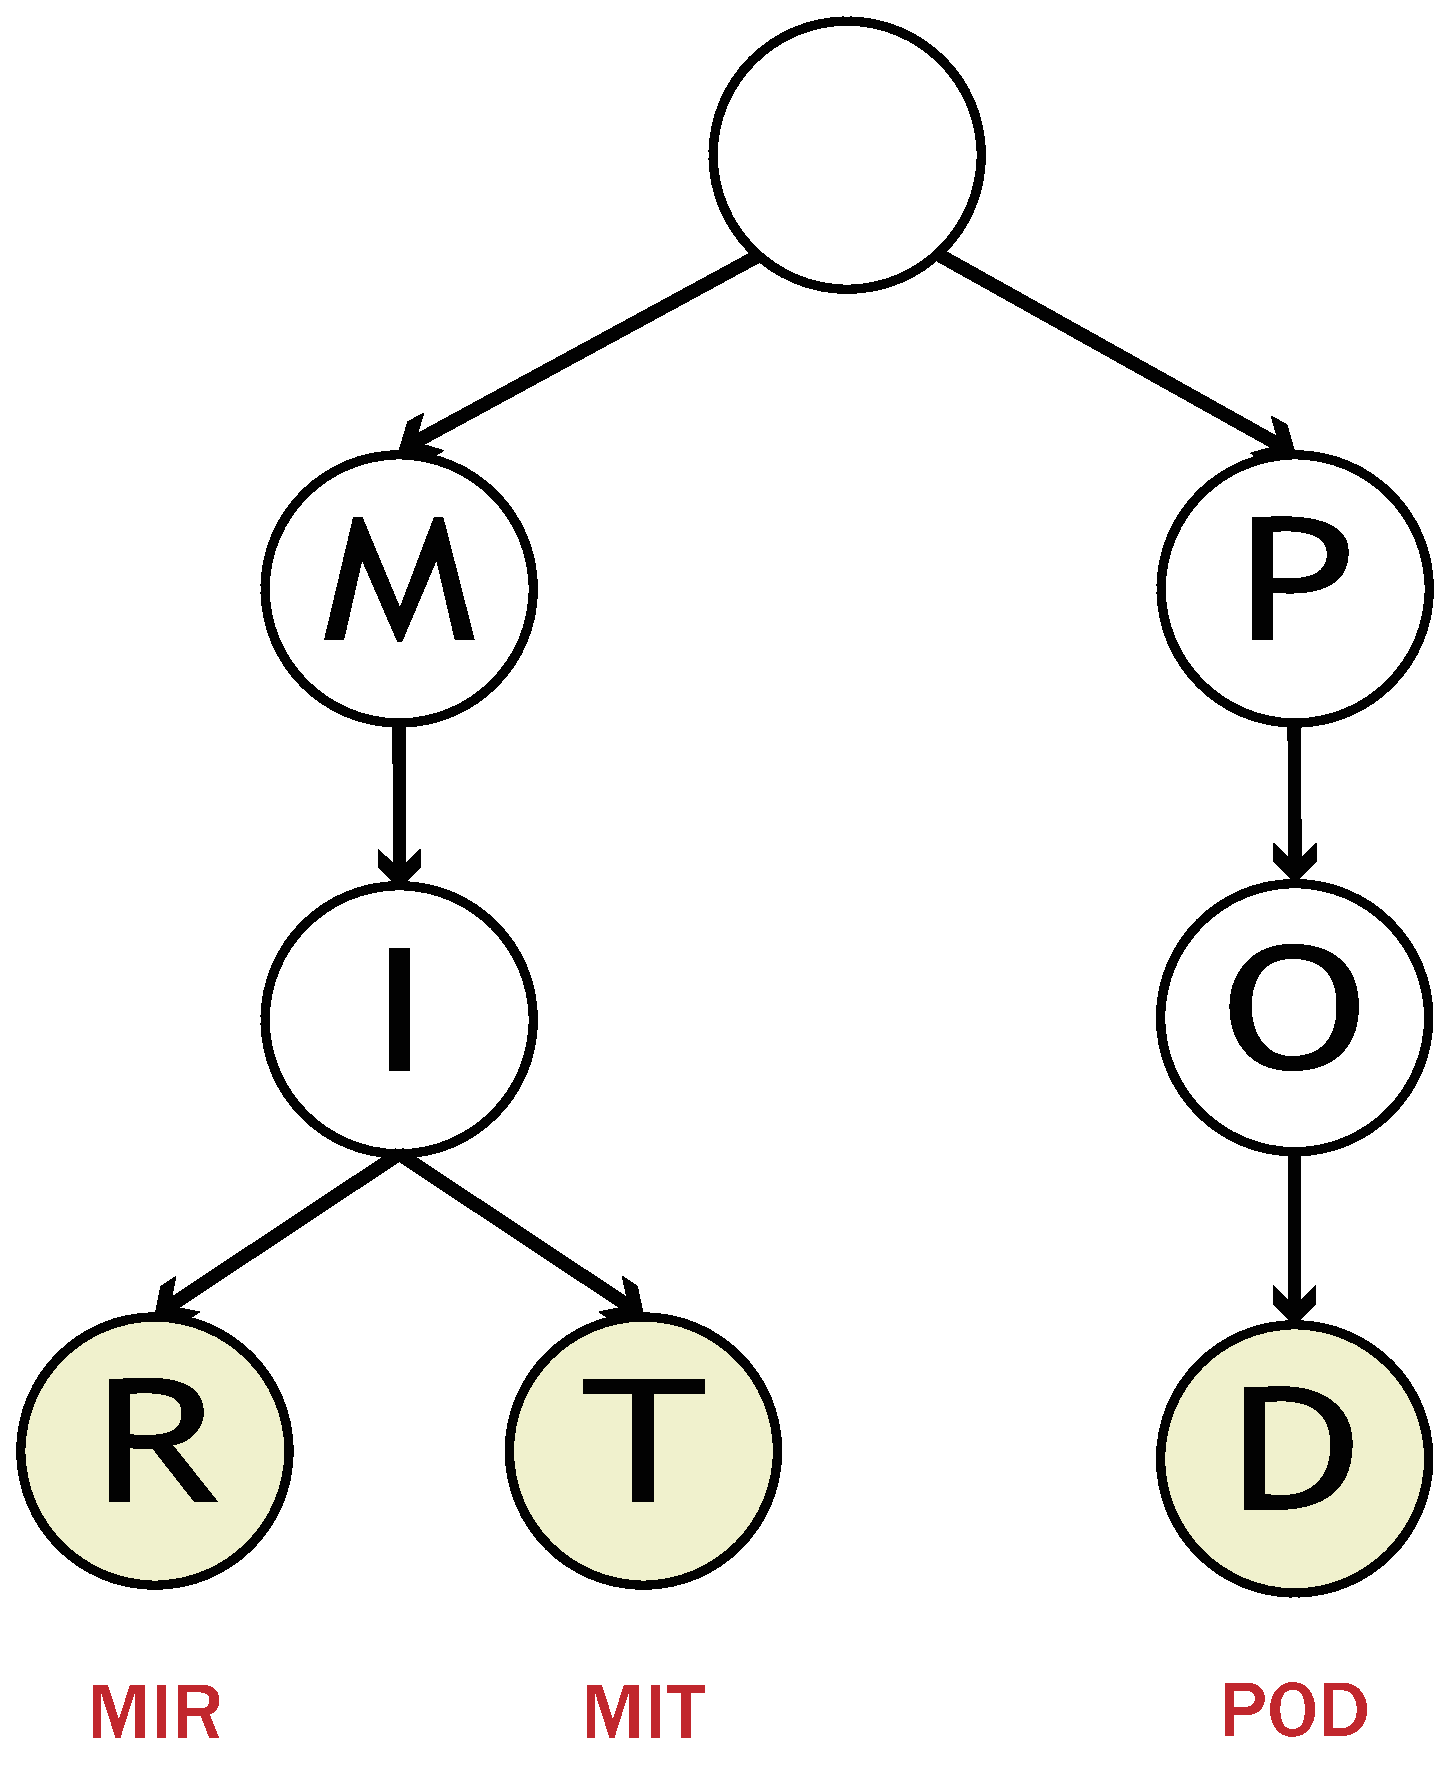
\includegraphics[width=0.40\textwidth]{radix_tree.eps}
  \caption{Primer radiks-stabla, gde su čvorovi koji sadrže vrednosti
    obeleženi žutom bojom, a crvenom bojom su napisani ključevi koji im
    odgovaraju}
  \label{fig:radix}
\end{figure}

Ukoliko bi se u primeru na
slici~\ref{fig:radix} dodao par sa ključem \texttt{PO},
stablo ne bi menjalo svoju strukturu, već
bi se samo čvoru \texttt{O} dodala nedostajuća vrednost.
Pri dodavanju para sa ključem \texttt{MAK}, pretraga bi prilikom prolaska
kroz stablo došla do čvora \texttt{M} i tu bi stala,
pošto ne postoji dete \texttt{A}. Tada se dodaje novo podstablo
čvoru \texttt{M}, gde se dobija novo stablo kao na slici~\ref{fig:radix2}.


Ovom metodom grupisanja sličnih ključeva u
istom podstablu rezultuje vremenskom složenošću čitanja, umetanja i brisanja
elemenata koja ne zavisi od broja elemenata
unetih u strukturu niti od veličine same strukture, već od
dužine ključa u njegovoj binarnoj reprezenaciji. Iako je vremenska složenost linearna,
osobina da efikasnost ne zavisi od broja unetih elemenata je pogodna za primenu
u memorisanim bazama podataka. Prednost radiks-stabala je i u činjenici da ona,
za razliku od stabala pretrage, ne zahtevaju rebalansiranje zarad
održavanja visine stabla.

\begin{figure}[!h]
  \centering
  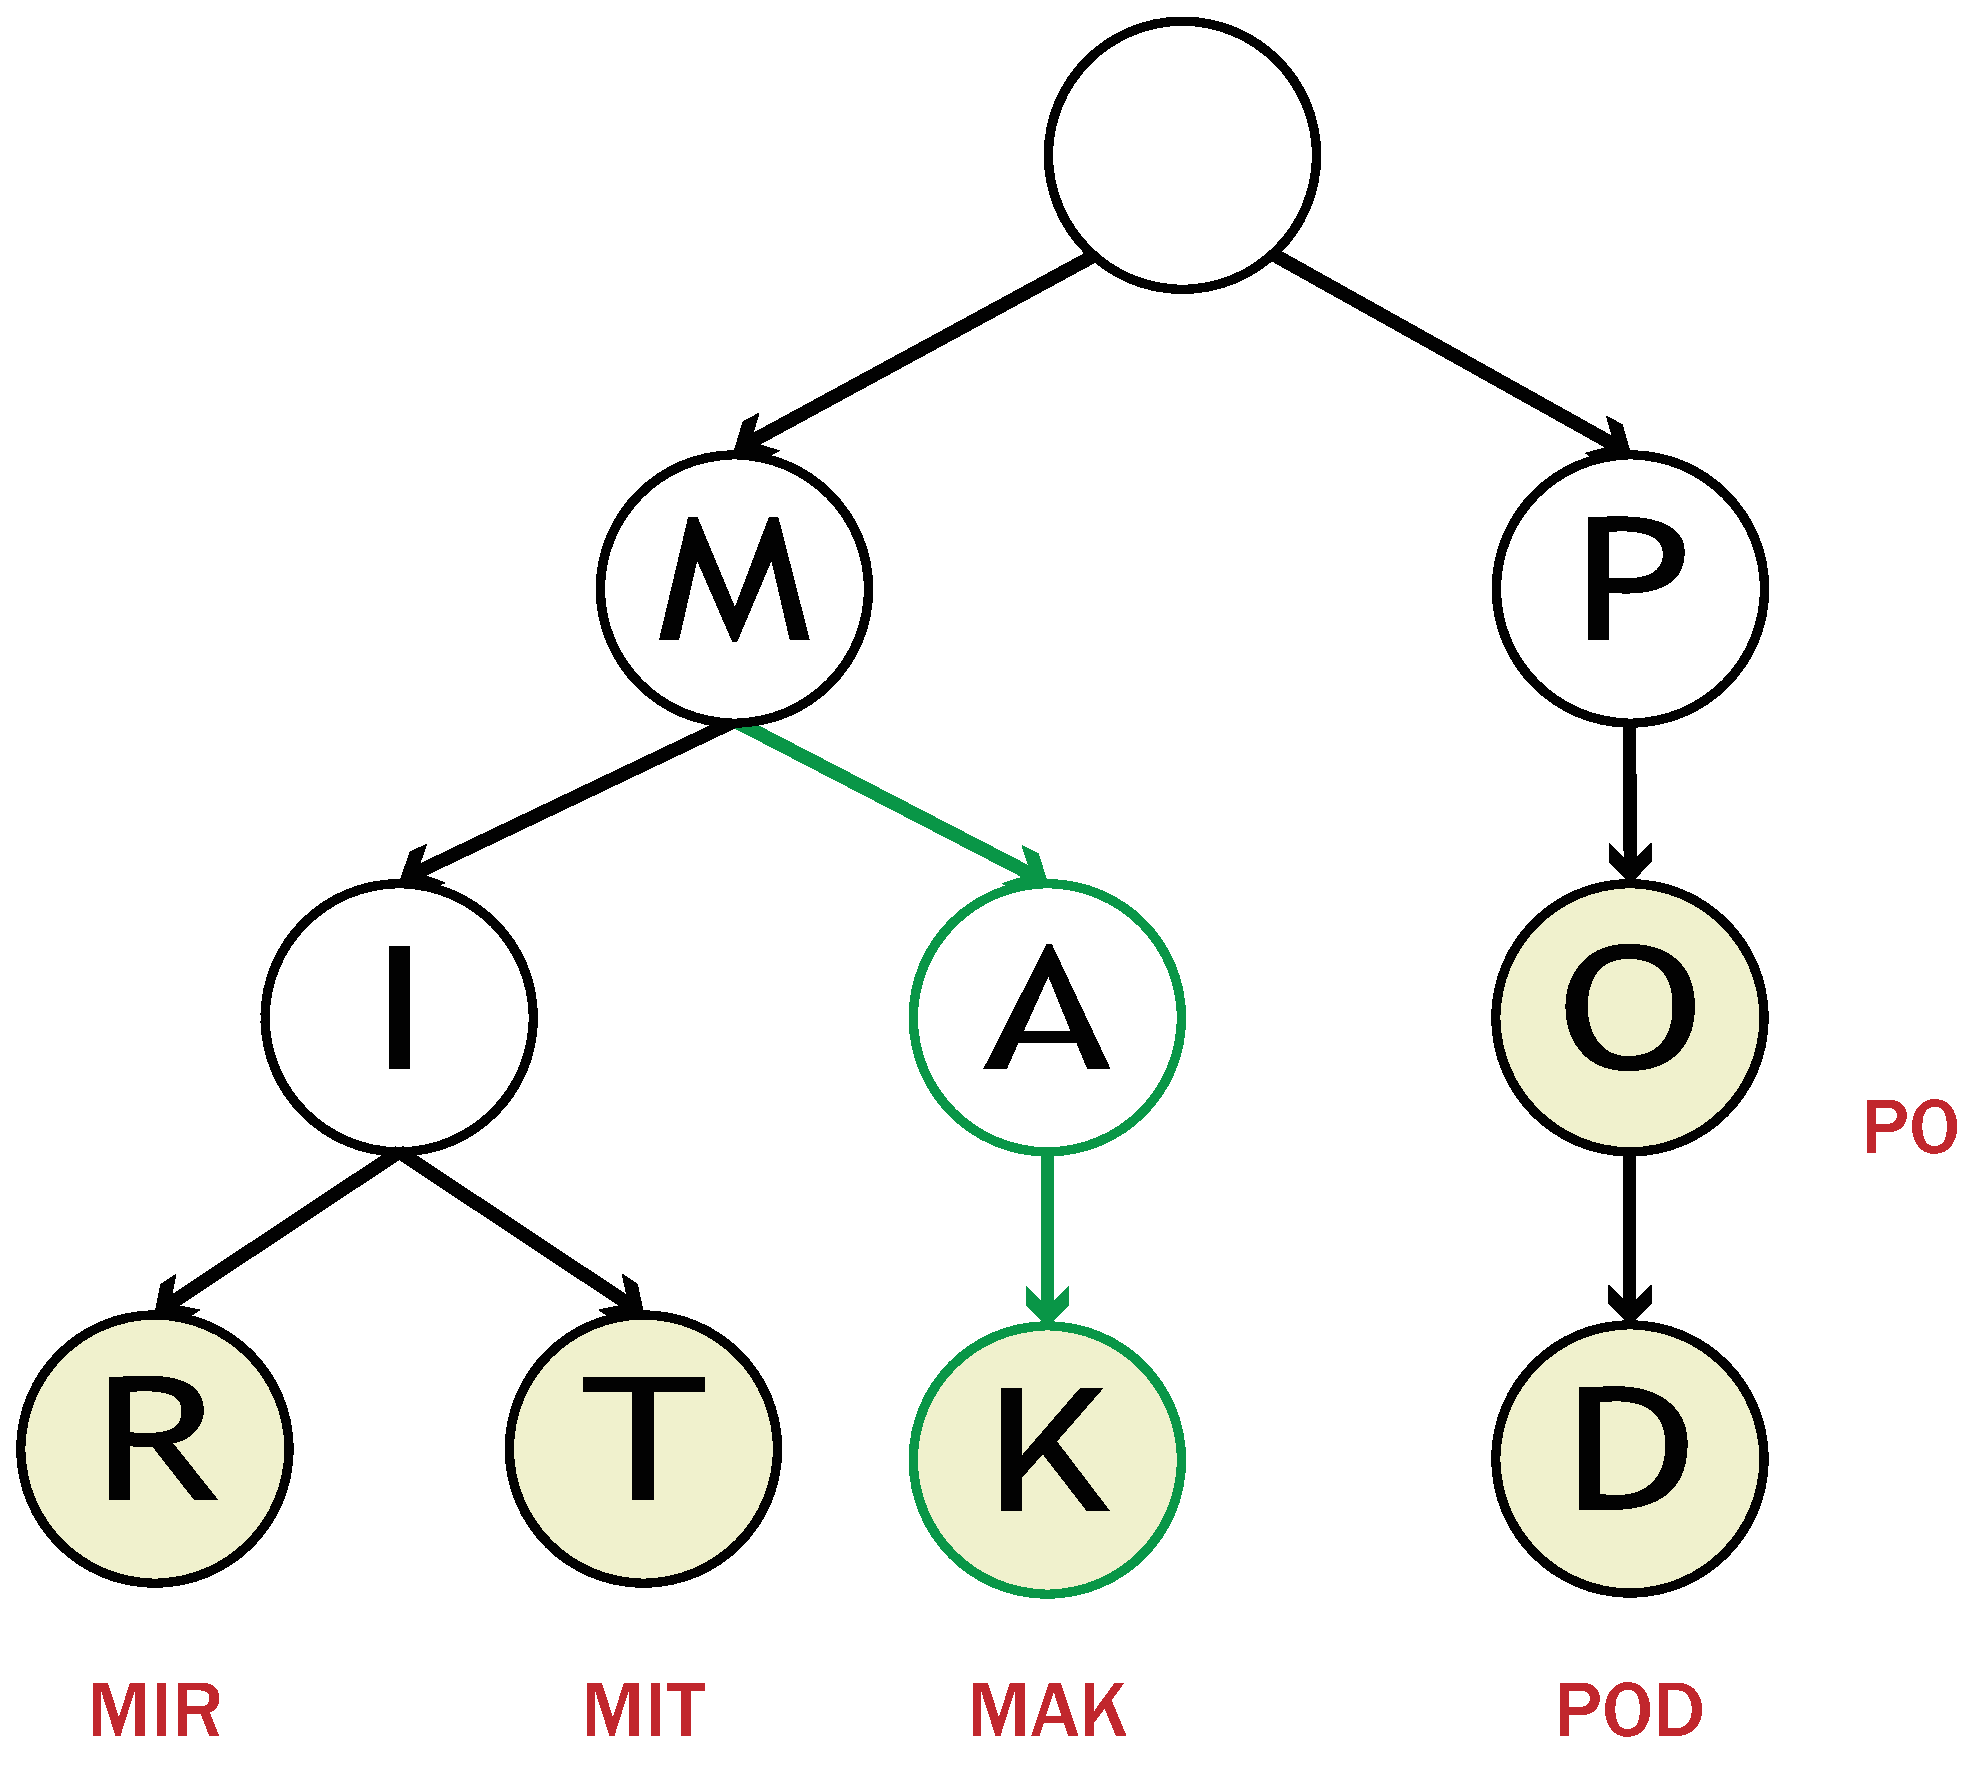
\includegraphics[width=0.55\textwidth]{radix_tree_2.eps}
  \caption{Radiks-stablo dobijeno dodavanjem ključeva \texttt{PO} i \texttt{MAK}}
  \label{fig:radix2}
\end{figure}

Problem koji se javlja kod radiks-stabala jeste prevelik utrošak memorije.
Ukoliko svaki čvor predstavlja jedan bajt ključa, to znači da
svaki čvor može imati, u najgorem slučaju, $ 2^{8} $ dece,
odnosno 256 pokazivača na decu.
Kako svaki čvor neće imati maksimalan broj dece, rezervisanje memorijskog prostora
za najgori slučaj rezultuje prekomernim korišćenjem memorije u prosečnom slučaju.
Lajs, Kemper i Nojman su, na IEEE internacionalnoj konferenciji inženjeringa
podataka 2013.\ godine, predstavili prilagodljiva radiks-stabla,
skraćeno nazvana \textbf{ART}~\cite{artful}
(engl. \emph{\textbf{A}daptive \textbf{R}adix \textbf{T}ree})
kao potencijalno novo rešenje, zato što ona dinamički
prilagođavaju veličinu unutrašnjih čvorova u odnosu na broj dece.
Na slici~\ref{fig:radix_v_art} je ilustrovana razlika između radiks-stabla i
prilagodljivog radiks-stabla.

\hspace{10pt}
\begin{figure}[!h]
  \centering
  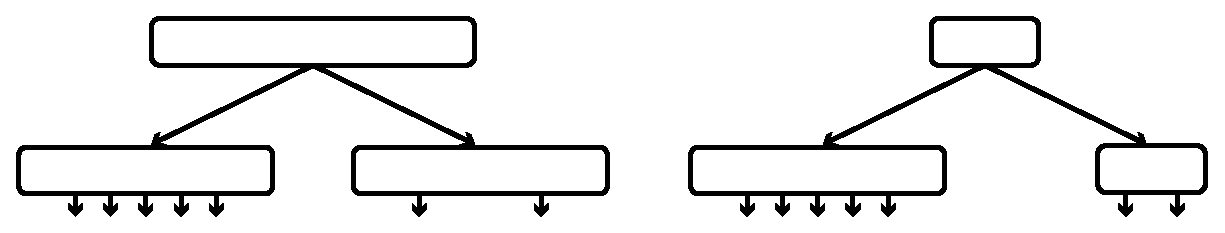
\includegraphics[width=0.95\textwidth]{radix_v_art.eps}
  \caption{
    Radiks-stablo (levo) i prilagodljivo radiks-stablo (desno)
  }
  \label{fig:radix_v_art}
\end{figure}

\section{Struktura prilagodljivih radiks-stabala}~\label{sec:struktura_art}

Čvorovi radiks-stabla ne moraju nužno memorisati jedan bajt ključa.
Broj bitova koji unutrašnji čvorovi memorišu se naziva \textbf{raspon} (engl. \emph{span}).
To znači da, u svom osnovnom obliku, radiks-stabla imaju visinu koja zavisi od
dužine ključa $k$ i od raspona $s$, i ona iznosi $ \lceil \frac{k}{s} \rceil $.

Odabir raspona ima uticaja i na vremensku i na memorijsku složenost
radiks-stabla. Ukoliko je raspon mali, onda je potencijalni broj dece po
unutrašnjem čvoru manji, pa je memorija bolje iskorišćena. S druge strane,
visina stabla je velika, te su operacije na stablu sporije.
I suprotno važi: ukoliko je raspon veliki,
onda je visina stabla mala i operacije se vrše brzo, ali je memorijska složenost
prevelika. Implementacije radiks-stabala GPT~\cite{gpt} i LRT~\cite{lrt}
koriste četiri, odnosno šest bitova raspona.

Na slikama~\ref{fig:radix_span2}
i~\ref{fig:radix_span3} su prikazani primeri radiks-stabala sa vrednostima
raspona 2 i 3. U oba stabla su uneti parovi sa istim šestobitnim ključevima:
\texttt{001110}, \texttt{001111} i \texttt{100001}.


\begin{figure}[!h]
  \centering
  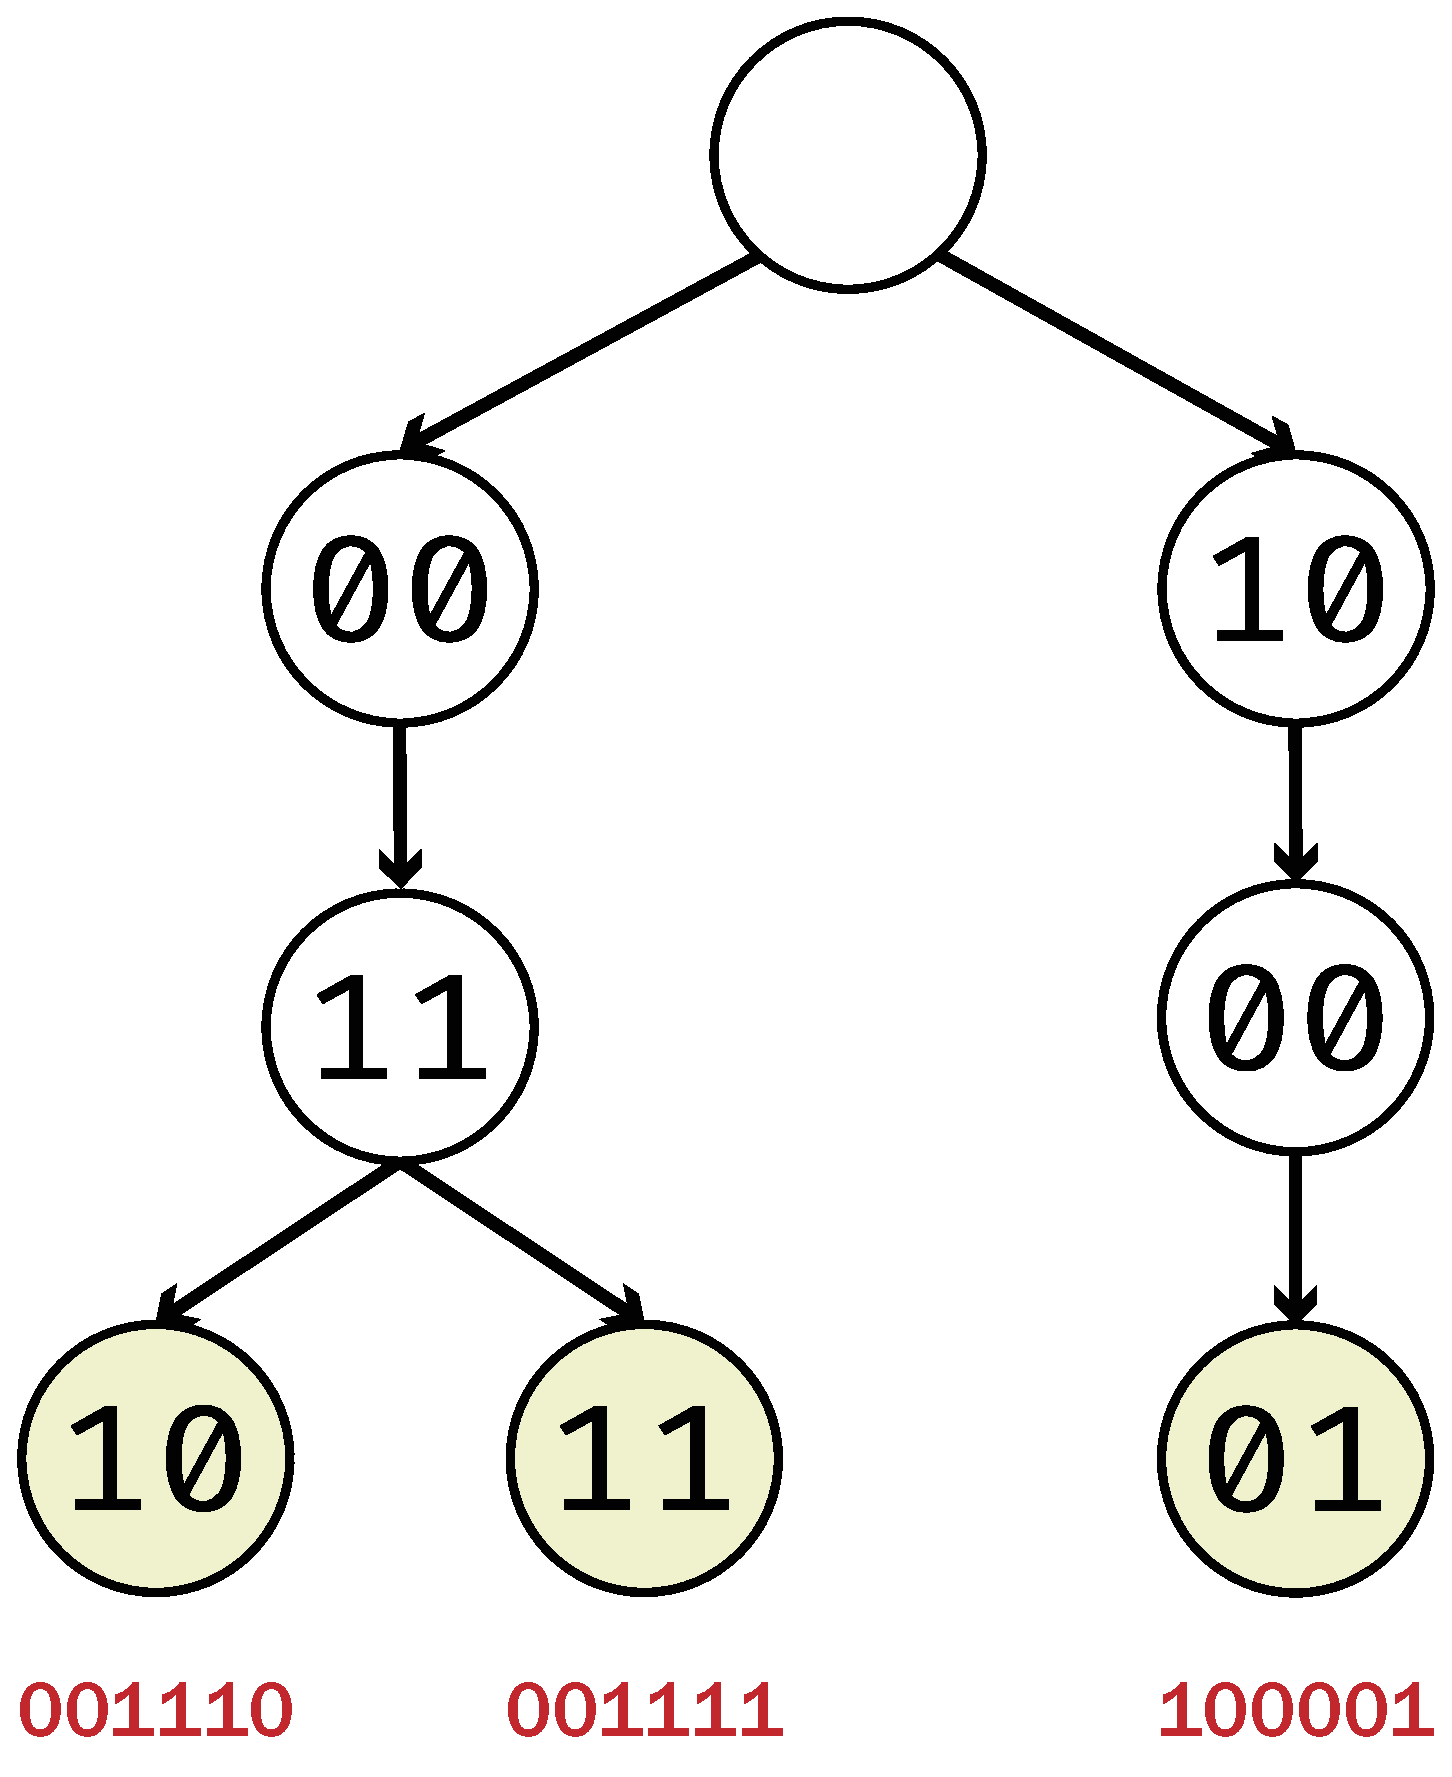
\includegraphics[width=0.40\textwidth]{radix_span2.eps}
  \caption{Primer radiks-stabla sa rasponom 2}
  \label{fig:radix_span2}
\end{figure}

\begin{figure}[!h]
  \centering
  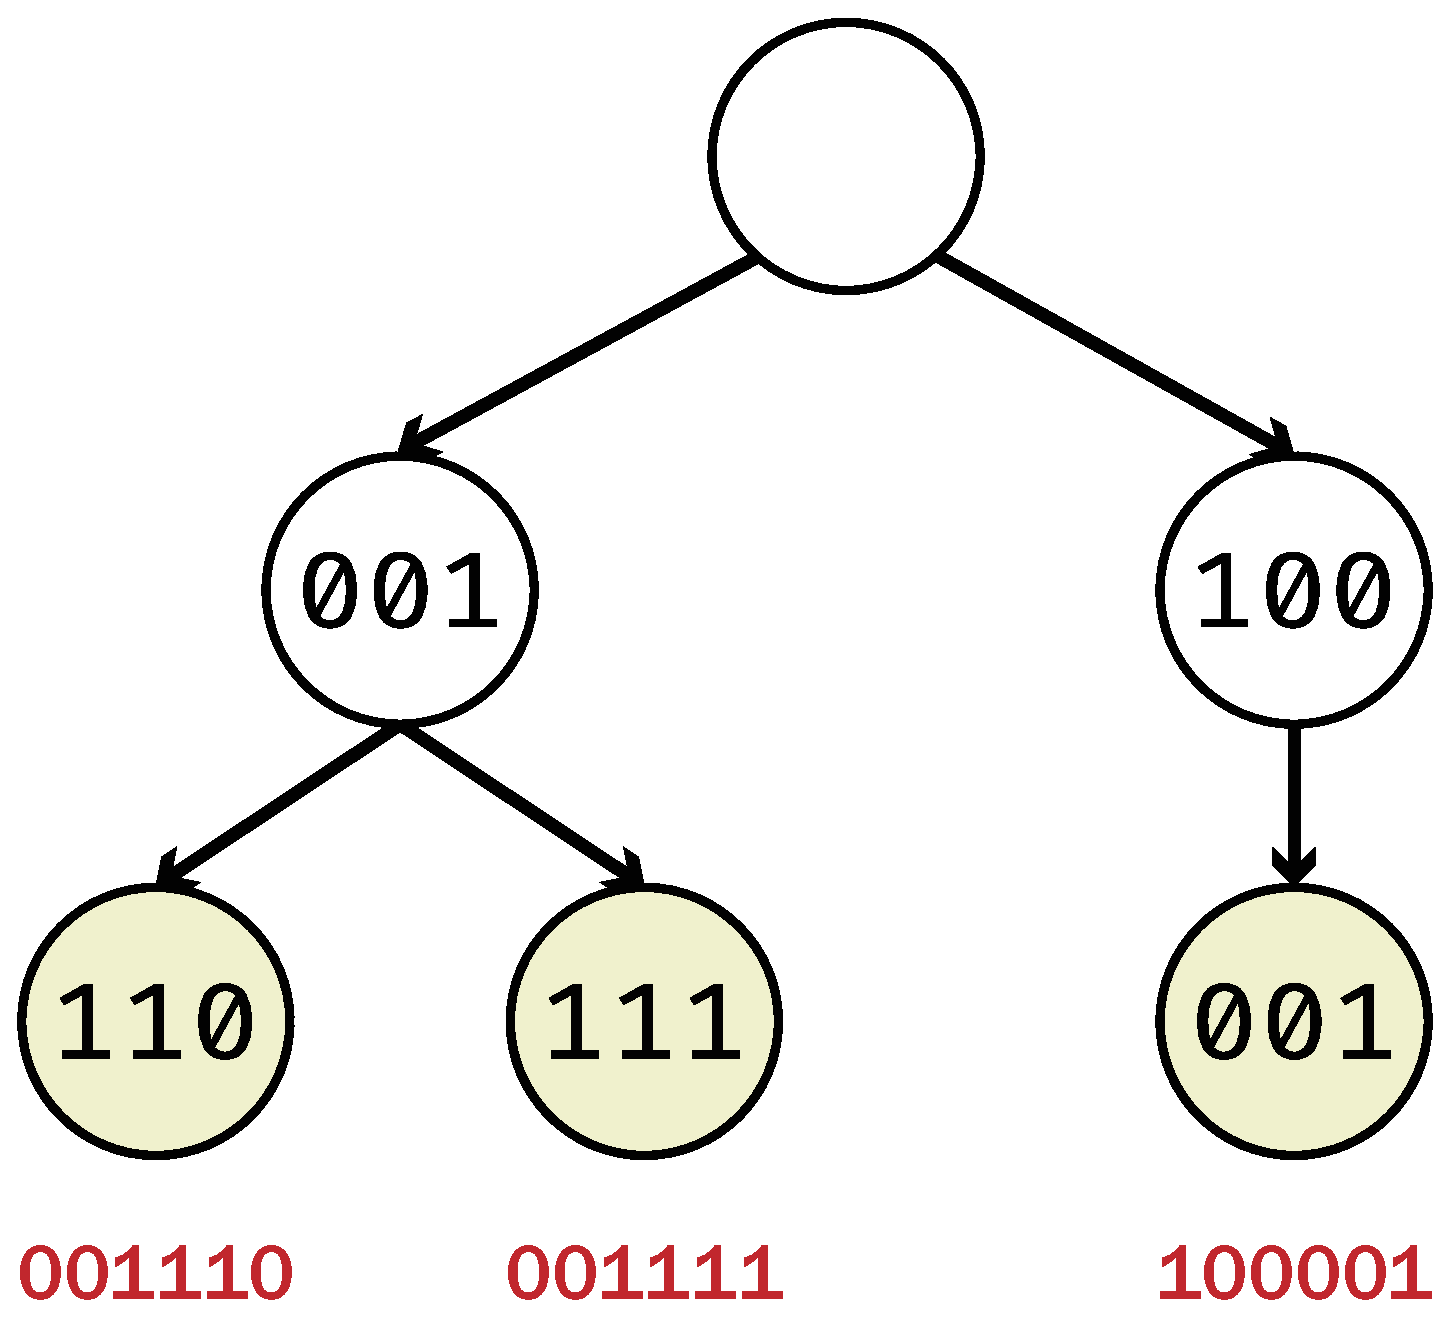
\includegraphics[width=0.42\textwidth]{radix_span3.eps}
  \caption{Primer radiks-stabla sa rasponom 3}
  \label{fig:radix_span3}
\end{figure}

ART ima raspon od osam bita, odnosno jedan bajt. Da bi se sprečila prekomerna
upotreba memorije, koriste se četiri različita tipa unutrašnjih čvorova u odnosu
na maksimalan broj pokazivača na decu, koji su ilustrovani na
slici~\ref{fig:radix_nodes}:

\begin{description}

  \item[Node4] Najjednostavniji oblik unutrašnjeg čvora
        i sastoji se od
        dva vektora dužine 4: vektor ključeva koji sadrži bajtove ključa i
        vektor dece koji sadrži pokazivače na decu. Svaki element vektora
        ključeva odgovara elementu na istoj poziciji u vektoru dece.
        Budući da je vektor ključeva male veličine, on se pretražuje
        linearnom pretragom.
  \item[Node16] Koristi dva vektora dužine 16.
        Kao i kod \texttt{Node4}, elementi dva vektora su upareni.
        Kako su vektori većeg kapaciteta, tako linearna
        pretraga predstavlja nezanemarljiv utrošak procesorskog
        vremena. Zbog toga se koriste pomenute SIMD instrukcije koje su
        hardverski podržane od strane procesora i koje
        omogućavaju paralelnu pretragu svih elemenata vektora ključeva.
  \item[Node48]
        Koristi vektor ključeva koji sadrži maksimalnih 256 elemenata
        kao i vektor dece koji sadrži 48 elemenata.
        Bajtovi pretrage su implicitno pohranjeni kao indeksi
        vektora ključeva. U vektoru ključeva se nalaze indeksi elemenata
        vektora dece, koji odgovaraju datom bajtu pretrage.
        SIMD instrukcije se u ovom slučaju ne mogu koristiti zato što su
        SIMD vektori hardverski ograničeni po broju bitova koje mogu sadržati.
  \item[Node256] Sastoji se od samo jednog vektora koji sadrži pokazivače na decu,
        dok se bajtovi pretrage implicitno čuvaju kao indeksi vektora
        dece. Ovaj tip koristi više memorije od \texttt{Node48},
        zato što pokazivači zauzimaju više memorije od čuvanja indeksa
        koji se predstavljaju jednim bajtom.
\end{description}

\begin{figure}[!h]
  \centering
  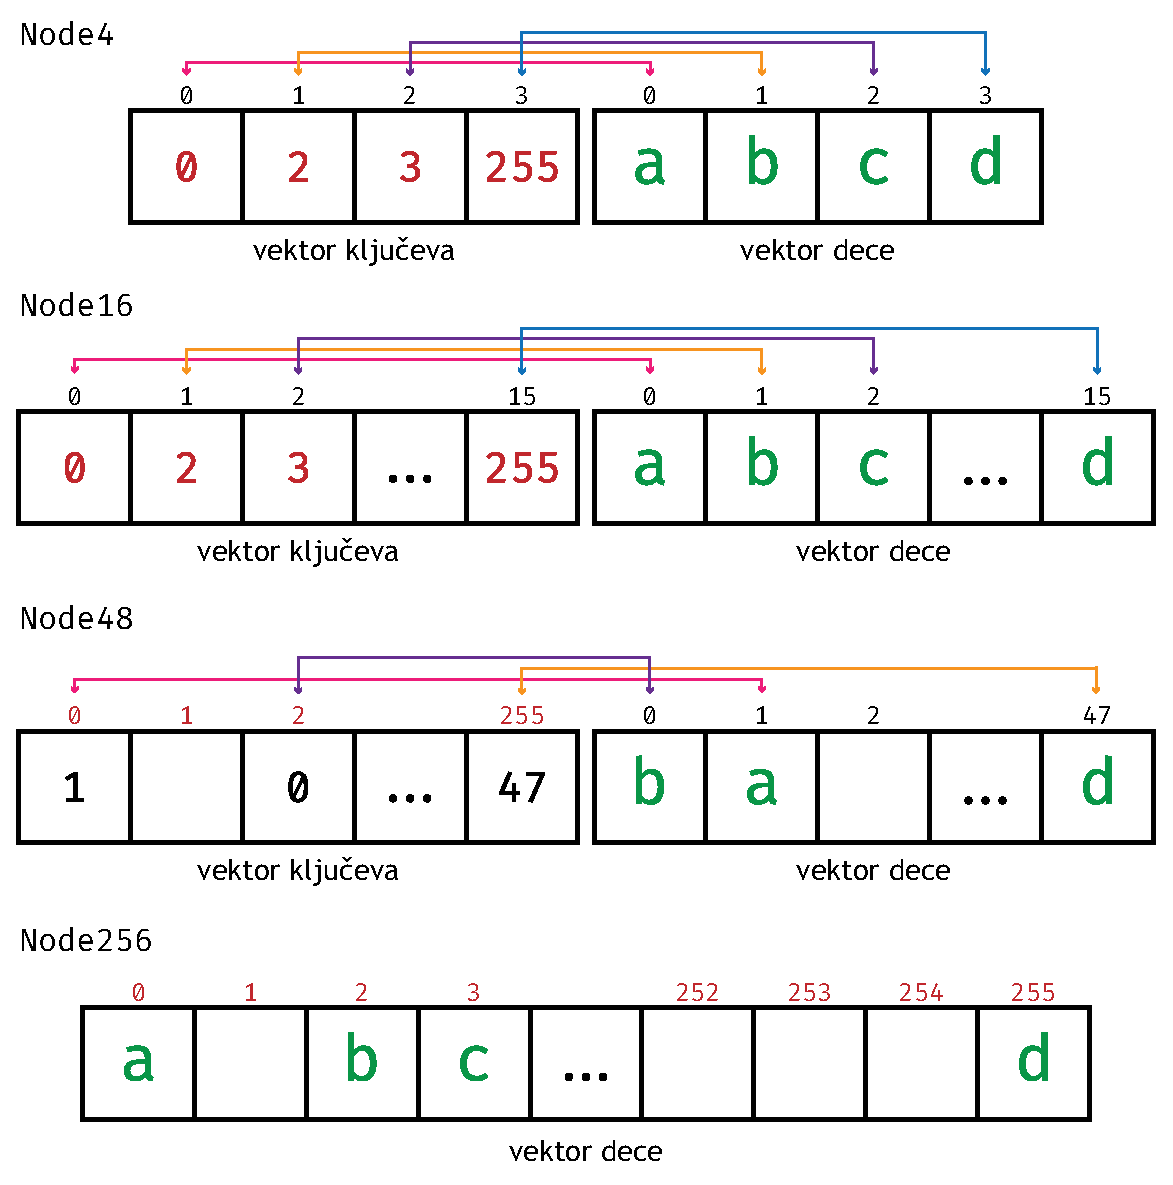
\includegraphics[width=0.75\textwidth]{radix_nodes.eps}
  \caption{Četiri tipa unutrašnjeg čvora u strukturi ART.\
    Strelicama su povezani
    odgovarajući parovi elemenata u vektorima ključeva i dece. Sa tri tačke
    su obeleženi elementi koji nisu prikazani na slici. Crvenom bojom su obeleženi
    bajtovi pretrage, dok su pokazivači na decu predstavljeni zelenim slovima.
  }
  \label{fig:radix_nodes}
\end{figure}

\noindent Ukoliko čvor popuni svoj kapacitet, onda se on transformiše u naredni
čvor po veličini.

\section{Memorijska optimizacija unutrašnjih čvorova}

Parcijalni ključ čvora radiks-stabla se odnosi na deo ključa
koji taj čvor reprezentuje.
Nadovezujući parcijalne ključeve čvorova na putu od korena stabla
do bilo kog drugog čvora predstavlja konkretan ključ tog čvora.
U svom osnovnom obliku, u radiks-stablu su parcijalni ključevi
fiksirane dužine.

Da bi se memorijska iskorišćenost optimizovala, koristi se metoda
\textbf{sažimanja puteva} (engl. \emph{path compression}) koja udružuje unutrašnje
čvorove koji imaju samo jedno dete sa tim detetom, ukoliko roditelj ne sadrži
vrednost. Prilikom udruživanja dva čvora,
parcijalni ključevi tih čvorova se nadovezuju.
Kako broj bitova parcijalnih ključeva reprezentuju nije više
fiksirana veličina, svaki bit izvan raspona stabla se mora čuvati
eksplicitno. Postoje dva metoda čuvanja parcijalnih ključeva unutrašnjih
čvorova:

\begin{description}
  \item[Pesimističan] Svaki unutrašnji čvor ima odgovarajući vektor
        u kome se čuvaju bitovi parcijalnog ključa. Primer pesimističnog
        sažimanja puteva dat je na slici~\ref{fig:radix_compression},
        gde je sažimanje puteva primenjeno na primeru sa
        slike~\ref{fig:radix2}.
  \item[Optimističan] Svaki unutrašnji čvor čuva informaciju o dužini
        parcijalnog ključa $d$. Prilikom pretraživanja stabla preskače se
        $d$ bitova ključa pretrage bez provere jednakosti,
        i pretraga se nastavlja dalje.
        Kad pretraga stigne do lista, tada se ceo ključ proverava.
\end{description}


\begin{figure}[!h]
  \centering
  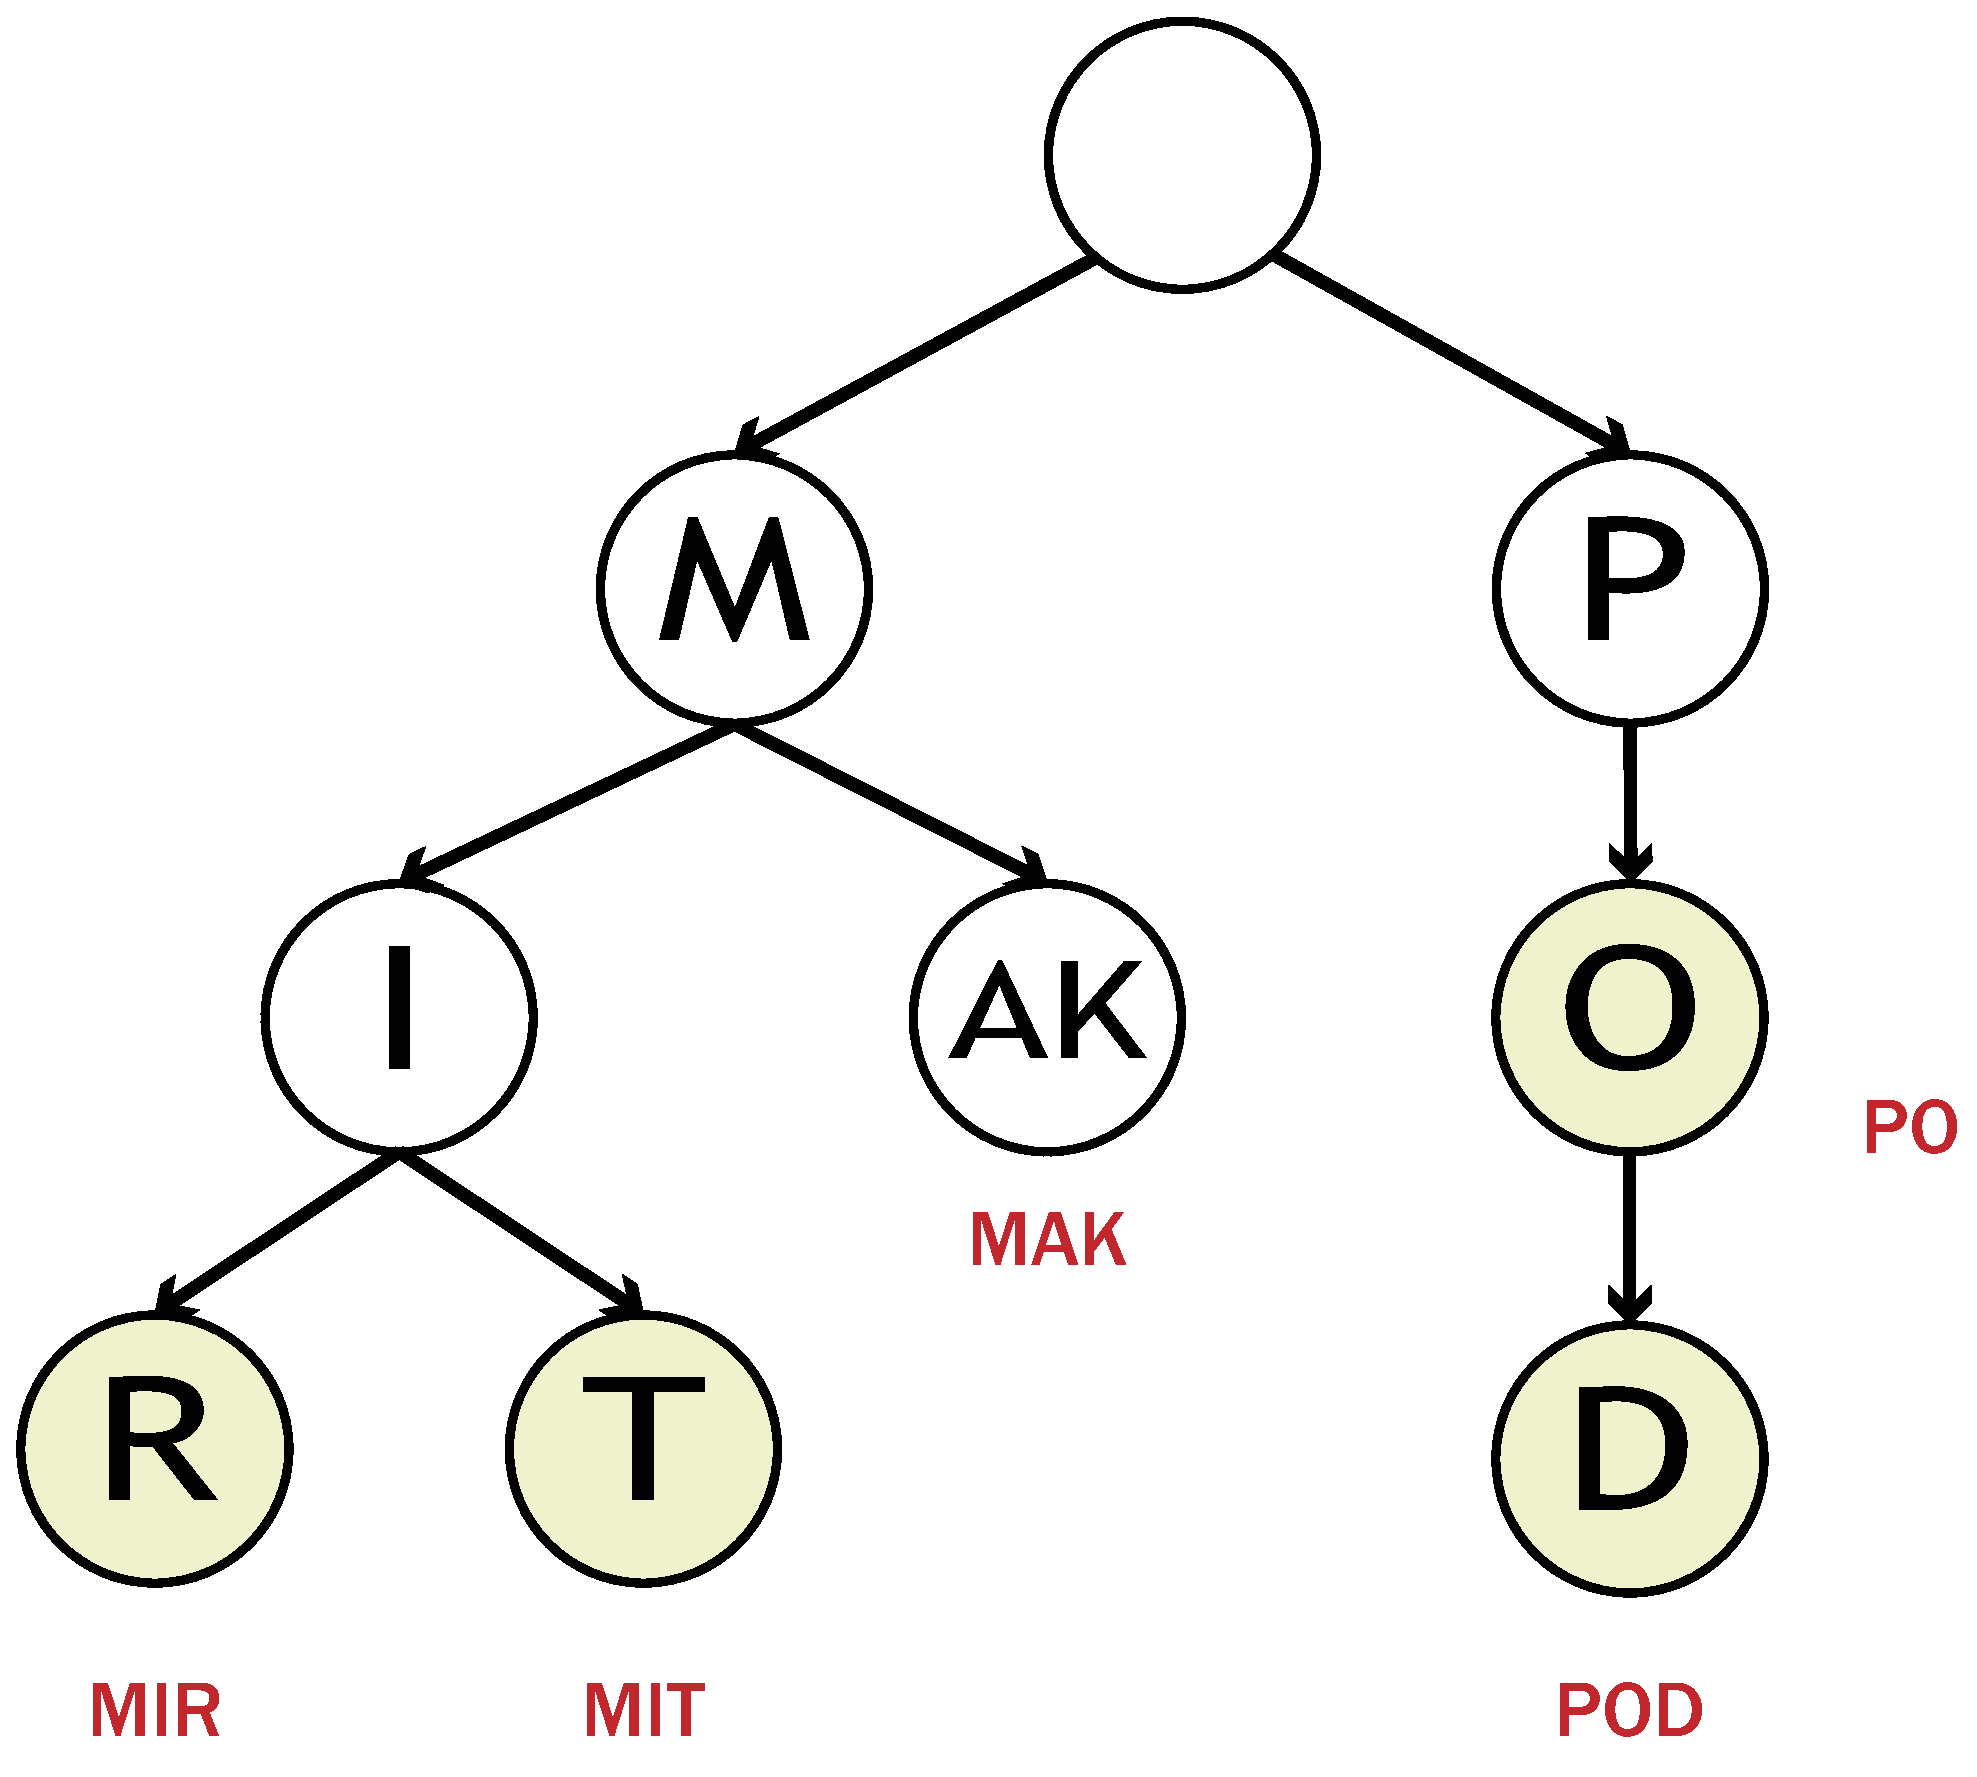
\includegraphics[width=0.55\textwidth]{radix_compression.eps}
  \caption{Pesimistično sažimanje puteva radiks-stabla, gde su samo
    čvorovi \texttt{A} i \texttt{K}, kao i \texttt{P} i \texttt{O} sažeti,
    dok \texttt{PO} i \texttt{D} nisu, jer čvor \texttt{PO}
    sadrži vrednost}
  \label{fig:radix_compression}
\end{figure}

Pesimističan metod daje brzu proveru korektnosti putanje, ali sa sobom nosi
povećanu potrošnju memorije. Uz to, može doći i do fragmentacije
memorije kada se vektori parcijalnih ključeva menjaju.
Nasuprot tome, optimističan metod nema
problema vezanih za memoriju, ali pretraga može da ode pogrešnom granom zato što se
nije dokazala jednakost parcijalnih ključeva. Tada se
pretraga mora vratiti unazad, što otežava implementaciju i ima negativan
uticaj na performanse. Postoji i hibridan način čuvanja parcijalnih ključeva,
gde se u unutrašnjim čvorovima čuva fiksni broj bajtova parcijalnog ključa.
Sve preko unapred određenog broja bajtova tog vektora se ne memoriše,
već se koristi optimističan metod čuvanja.

\section{Algoritmi pretrage i umetanja}

U svom radu iz 2013.\ godine, autori prilagodljivih radiks-stabala su
objavili i algoritme pretrage i umetanja. Ovi algoritmi su veoma slični
algoritmima za radiks-stabla u osnovnom obliku, i zato će biti navedeni
i objašnjeni samo algoritmi za rad sa strukturom podataka ART.\
Algoritam pretrage je dat na listingu~\ref{art:algoritam_pretrage}.

\begin{lstlisting}[language=C++,
                   caption={Algoritam pretrage strukture podataka ART},
                   label={art:algoritam_pretrage}]
search(node, key, depth):
    if node == NULL
        return NULL
    if isLeaf(node)
        if leafMatches(node, key, depth)(*@\label{line:leafMatches}@*)
            return node
        return NULL
    if checkPrefix(node, key, depth) != node.prefixLen
        return NULL
    depth += node.prefixLen
    next = findChild(node, key[depth])
    return search(next, key, depth + 1)
\end{lstlisting}

Funkcija \texttt{search} ima tri parametra: trenutni čvor pretrage, ključ
pretrage i dubinu trenutnog čvora. Kako je ovaj algoritam rekurzivan,
prvo se proverava bazni slučaj kada je trenutni čvor ili prazan ili
list, gde se rezultat vraća samo ukoliko je čvor list i ključ u tom listu
se poklapa sa ključem pretrage. U drugom slučaju, ako je pretraga trenutno
u unutrašnjem čvoru, prvo se proverava poklapanje parcijalnog prefiksa
u čvoru u liniji~\ref{line:leafMatches} i pretraga se završava ako dođe
do nejednakosti parcijalnih ključeva. Zatim se koriguje dubina pretrage
promenljivom \texttt{depth},
zato što se on odnosi na indeks bajtova koji se
porede u tom trenutku.
Na kraju, nalazi se idući čvor funkcijom \texttt{findChild} prosleđivanjem
trenutnog čvora i odgovarajućeg bajta i pretraga se
nastavlja rekurzivno. Isti algoritam pretrage se može primeniti i za
radiks-stabla u osnovnom obliku. Algoritam funkcije
\texttt{findChild} je dat na listingu~\ref{art:algoritam_findChild}.

\begin{lstlisting}[language=C++,
                   caption={Algoritam pronalaska idućeg čvora pretrage},
                   label={art:algoritam_findChild}]
findChild(node, byte):
    if node.type == Node4
        for (i = 0; i < node.count; i = i + 1)
            if node.key[i] == byte
                return node.child[i]
        return NULL
    if node.type == Node16
        for (i = 0; i < node.count; i = i + 1)
            key = _mm_set1_epi8(byte)
            cmp = _mm_cmpeq_epi8(key, node.key)
            mask = (1 << node.count) - 1 (*@\label{line:mask}@*)
            bitfield = _mm_movemask_epi8(cmp) & mask
            if bitfield
                return node.child[ctz(bitfield)]
            else
                return NULL
    if node.type == Node48
        if node.childIndex[byte] != EMPTY
            return node.child[node.childIndex[byte]]
        else
            return NULL
    if node.type == Node256
        return node.child[byte]
\end{lstlisting}

Naredni čvor se nalazi na četiri različita načina, u odnosu na
tip trenutnog čvora koji je poslat kao parametar funkciji
\texttt{findChild}:

\begin{description}
  \item[Node4] Naredni čvor se nalazi linearnom
        pretragom svih elemenata
        vektora ključeva.
  \item[Node16] U ovom slučaju se koriste SIMD instrukcije.
        Prvo se, pomoću funkcije \texttt{\_mm\_set1\_epi8} inicijalizuje
        SIMD vektor od 128 bita, odnosno, 16 elemenata veličine jednog bajta. Svi
        elementi tog vektora biće jednaki bajtu koji je unet kao parametar.
        Posle inicijalizacije se porede svi elementi novog vektora i
        vektora ključeva trenutnog čvora funkcijom
        \texttt{\_mm\_cmpeq\_epi8}. Kao rezultat se dobija vektor iste
        dužine, ali čiji elementi su binarne vrednosti \texttt{0}
        i \texttt{11111111}, u zavisnosti da li su elementi na odgovarajućoj
        poziciji jednaki ili ne. U liniji~\ref{line:mask} se pravi
        maska zato što vektor elemenata nije nužno pun, ali postoji
        mogućnost poklapanja bajta pretrage sa bajtovima koji nisu
        u upotrebi, zato što SIMD vektor mora biti inicijalizovan
        u potpunosti prilikom njegovog definisanja.
        Maska je veličine
        32 bita, pa se vektor \texttt{cmp} šalje funkciji
        \texttt{\_mm\_movemask\_epi8} koja vraća 32-bitnu vrednost
        gde je svaki element vektora (ukupno ih je 32) reprezentovan
        svojim najznačajnijim bitom. Kada se primeni maska na dobijenu
        vrednost, dobija se 32-bitna vrednost \texttt{bitfield},
        a ključ se nalazi u mestu kojem odgovara bit sa vrednošću
        1. Da bi se našao indeks prvog bita sa vrednošću 1, koristi
        se funkcija \texttt{ctz}
        (engl.\ \textit{\textbf{c}ount \textbf{t}railing \textbf{z}eros})
        koja broji nule na kraju vrednosti zapisane u binarnom
        sistemu.
  \item[Node48] Indeks narednog čvora je upisan u vektoru
        \texttt{childIndex} koji ima 256 elemenata, za svaku
        vrednost bajta pretrage. Ukoliko vrednost za
        taj ključ nije uneta,
        u vektor \texttt{childIndex} se piše fiksirana
        vrednost \texttt{EMPTY} koja je veća od 48 (maksimalnog
        broja elemenata u nizu dece).
  \item[Node256] Koristi se niz maksimalne veličine od 256 elemenata
        gde se bajt ključa direktno koristi za indeksiranje.
\end{description}

U slučaju osnovnih radiks-stabala, algoritam \texttt{findChild}
je sličan \texttt{Node256} grani iz
algoritma sa listinga~\ref{art:algoritam_findChild} koja
se prilagođava za različite vrednosti raspona $s$.
Veličina vektora koji se nalaze u unutrašnjim
čvorovima je uslovljena odabirom vrednosti raspona
i ona iznosi $2^{s}$.

Algoritam za umetanje novih parova ključ-vrednost u stablo je dat
na listingu~\ref{art:algoritam_insert}, dok je algoritam brisanja
parova, po rečima autora, simetričan ovom algoritmu. Ponovo je u pitanju
rekurzivni algoritam, te se prvo obrađuje bazni slučaj, odnosno kad
se praznom podstablu dodaje list. Ako je čvor kome se dodaje
element list, onda se pravi novi unutrašnji čvor funkcijom
\texttt{makeNode4} koji će da sadrži čvor koji se dodaje
kao i stari list. Pre toga, mora se utvrditi dužina prefiksa
u petlji u liniji~\ref{line:prefix_len}.

Ukoliko stablo nije prazno, niti je u pitanju list, onda je
prosleđeni čvor unutrašnji. Ako prefiks unutrašnjeg
čvora ne odgovara traženom ključu, onda dolazi do račvanja
stabla na dve grane gde se ponavlja slična procedura
kao i kod stabla koje sadrži samo jedan list. Na kraju, ako se
prefiksi poklapaju, onda se traži sledeći čvor gde bi se
pretraga mogla nastaviti. Ako naredni čvor u pretrazi postoji,
onda se pretraga rekurzivno nastavlja. U suprotnom, pretraga se
zaustavlja i novi list se dodaje trenutnom unutrašnjem čvoru.
Trenutni unutrašnji čvor može biti popunjen, pa se njegov
kapacitet mora proširiti pretvaranjem trenutnog
unutrašnjeg čvora u sledeći čvor u hijerarhiji funkcijom
\texttt{grow} (iz \texttt{Node4}
u \texttt{Node16}, iz \texttt{Node16} u \texttt{Node48} ili
iz \texttt{Node48} u \texttt{Node256}). Funkcija \texttt{grow}
je jedina suštinska razlika između algoritma sa
listinga~\ref{art:algoritam_insert} i algoritma za umetanje u
radiks-stablo i njena implemenacija zavisi od specifičnosti
konkretnog programskog jezika u kome se ona implementira.
Usled toga, funkcija \texttt{grow} će
biti prikazana u narednom poglavlju, gde se opisuje
implemenacija strukture ART u okviru programskog jezika
\textit{Rust}.

\begin{lstlisting}[language=C++,
                   caption={Algoritam umetanja novih elemenata u stablo},
                   label={art:algoritam_insert}]
insert (node, key, leaf, depth):
 if node == NULL
    replace(node, leaf)
    return
 if isLeaf(node)
    newNode = makeNode4()
    key2=loadKey(node)
    for (i = depth; key[i] == key2[i]; i = i + 1) (*@\label{line:prefix_len}@*)
        newNode.prefix[i - depth] = key[i]
    newNode.prefixLen = i - depth
    depth = depth + newNode.prefixLen
    addChild(newNode, key[depth], leaf)
    addChild(newNode, key2[depth], node)
    replace(node, newNode)
    return
 p=checkPrefix(node, key, depth)
 if p != node.prefixLen
    newNode = makeNode4()
    addChild(newNode, key[depth + p], leaf)
    addChild(newNode, node.prefix[p], node)
    newNode.prefixLen = p
    memcpy(newNode.prefix, node.prefix, p)
    node.prefixLen = node.prefixLen-(p + 1)
    memmove(node.prefix,node.prefix + p + 1,node.prefixLen)
    replace(node, newNode)
    return
 depth = depth + node.prefixLen
 next = findChild(node, key[depth])
 if next
    insert(next, key, leaf, depth + 1)
 else
    if isFull(node)
        grow(node)
 addChild(node, key[depth], leaf)
\end{lstlisting}

Vremenska složenost funkcija \texttt{search} i \texttt{insert}
zavisi od dubine stabla, koje iznosi
$ \lceil \frac{k}{s} \rceil $. Kako je raspon $s$ konstantan i
iznosi osam bita, vremenska složenost je
$ \mathcal{O}(k) $, gde je $k$ dužina ključa.

\chapter{ART u programskom jeziku \textit{Rust}}
Implementacija prilagodljivih radiks-stabala podrazumeva
kreiranje strukture koja podržava četiri različite operacije:
umetanje (engl.\ \textit{insert}), ažuriranje (engl.\ \textit{update}),
pretraživanje (engl.\ \textit{find}) i brisanje (engl.\ \textit{delete})
parova ključ-vrednost.

Umetanje i menjanje parova se spaja u jednu funkciju koja umeće dati par
u strukturu ukoliko ne postoji drugi par sa istim ključem u toj strukturi.
U suprotnom, vrednost za taj par se ažurira i funkcija vraća staru vrednost.

Struktura koja predstavlja prilagodljiva radiks-stabla se zove \texttt{ARTree}
i data je u listingu~\ref{kod:artree}. Definisana je u datoteci \texttt{lib.rs},
gde su definisane sve osnovne strukture za rad sa prilagodljivim radiks-stablima.
U definiciju \texttt{ARTree} ulaze dva generička tipa: tip ključa i tip vredosti
parova koji se unose u stablo. Prvo polje strukture je \texttt{root}, koje se odnosi
na koren prilagodljivog radiks-stabla. Da je koren i jedino polje ove strukture,
kompilator ne bi dopustio korišćenje generičkog tipa \texttt{K} koje se ne pominje
unutar same strukture. Zbog toga, mora se koristiti tzv.\ \textbf{fantomski marker},
koji kao generički tip uzima \texttt{K}. Ovaj tip podataka se naziva ``fantomskim''
zato što ne koristi memoriju, već je samo vrsta indikatora za kompilator.

\begin{lstlisting}[language=Rust,
                   caption={Definicija strukture \texttt{ARTree}},
                   label={kod:artree}]
pub struct ARTree<K: ARTKey, V> {
    root: ARTLink<V>,
    _marker: PhantomData<K>,
}
\end{lstlisting}

U listingu~\ref{kod:artree} generički tip \texttt{K} ima svojsvo \texttt{ARTKey}.
Ovo svojstvo, dato na listingu~\ref{kod:artkey} je takođe definisano u
datoteci \texttt{lib.rs}.

\begin{lstlisting}[language=Rust,
                   caption={Definicija svojstva \texttt{ARTKey}},
                   label={kod:artkey}]
pub trait ARTKey {
    fn convert_to_bytes(self) -> Vec<u8>;
}
\end{lstlisting}

\texttt{ARTKey} sadrži samo jednu funkciju: funkciju koja može dati ključ
prevesti u vektor bajtova, odnosno \texttt{Vec<u8>}. Da bi se vrednost
bilo kog tipa mogla koristiti kao ključ u \texttt{ARTree}, taj tip mora prvo
implementirati ovo svojstvo. U datoteci \texttt{key.rs} su date
implementacije ovog svojstva za primitivne tipove (celi brojevi, brojevi zapisani
u pokretnom zarezu), kao i za niske. Funkcija standardne biblioteke
\texttt{to\_be\_bytes} je definisana za sve brojeve i ona prevodi brojeve u
njihovu reprezentaciju u bajtovima u \textit{big-endian}~\cite{endianness}
sistemu. \textit{Big-endian} se odnosi na poredak bajtova smeštenih u memoriji,
odnosno na činjenicu da su bajtovi u memoriji smešteni po značajnosti.
Funkcija \texttt{to\_be\_bytes} smešta bajtove u niz,
koji se mora prevesti u vektor funkcijom \texttt{into\_vec}.
Standardna biblioteka takođe sadrži odgovarajuću funkciju za prevođenje
niski u bajtove koja se naziva \texttt{into\_bytes}.

\section{Struktura čvorova}
Definicije tipova čvorova se nalaze u datoteci \texttt{node.rs}.
Osnovni tip čvora se naziva \texttt{ARTNode} i on je enumerator.

U definiciji strukture \texttt{ARTree} na listingu~\ref{kod:artree}
koren stabla ima tip~\texttt{ARTLink<V>}. Ovaj tip je
pseudonim tipa \texttt{Option<Box<ARTNode<V>>>} koji predstavlja
pokazivače na decu.
\texttt{Box} pokazivač je ovde neophodan zato što je \texttt{ARTNode}
rekurzivna struktura, i kompilator bez njega ne bi znao
koliko memorije treba rezervisati.

\texttt{ARTNode} razlikuje dve vrste čvorova: unutrašnje \texttt{Inner} i
listove \texttt{Leaf}. U \texttt{Leaf} se smešta struktura \texttt{ARTLeaf}
koja sadrži vrednost i ključ dok se u \texttt{Inner} se smeštaju tri podatka:
enumerator \texttt{ARTInnerNode}, parcijalni ključ i vrednost. Vrednost se ovde
nalazi u \texttt{Option} omotaču, jer unutrašnji čvorovi
ne moraju nužno imati vrednosti.

\texttt{ARTInnerNode} sadrži četiri vrste unutrašnjeg čvora:
\texttt{Inner4}, \texttt{Inner16}, \texttt{Inner48} i
\texttt{Inner256} gde su, redom, smeštene odgovarajuće strukture
\texttt{ARTInner4}, \texttt{ARTInner16}, \texttt{ARTInner48} i
\texttt{ARTInner256}. Struktura ovih čvorova se suštinski ne razlikuje od
njihovog opisa u sekciji~\ref{sec:struktura_art}, s tim da su dodati
podaci o dužini parcijalnog čvora i broju smeštene dece.
Svi pomenuti tipovi čvorova imaju jedan generičan
tip: tip vrednosti. Generičan tip ključa nije neophodan nakon njegovog
transformisanja u vektor bajtova.


% ------------------------------------------------------------------------------
\chapter{Zaključak}

% ------------------------------------------------------------------------------
% Literatura
% ------------------------------------------------------------------------------
\literatura

% ==============================================================================
% Završni deo teze i prilozi
\backmatter
% ==============================================================================

% ------------------------------------------------------------------------------
% Biografija kandidata
\begin{biografija}
  \textbf{Jovan Dmitrović} (\emph{Gornji Milanovac, 17.11.1995.})
\end{biografija}
% ------------------------------------------------------------------------------

\end{document}
